\section{Level Design}
In this section the sequences of the implemented level "Giant Chasm" are explained. The level is divided into 5 sequences.\\
Under the representative map of the section are listed all the dialogues belonging to that specific time section.

\subsection{Scope of the level}

\vspace*{0.5cm}

\begin{center}
	\begin{tabular}[c]{| p{6cm} | p{4cm} | p{3cm} |}
		\hline
		Section 1 &                & \\
		 - Entrance                   & 5 minutes                  & 8,33\%                 \\
		 - Democerberus Boss Room          & 10 minutes                  & 16,66\%                 \\
		 - External Ovest Side           & 5 minutes			                & 8,33\%	                  \\ \hline
		 Section 2 &                & \\
		 - External North Side                   & 2 minutes                  & 3,33\%                 \\
		 - External East Side          & 8 minutes                  & 13,33\%                 \\
		 - Internal North Side           & 5 minutes		                & 8,33\%                  \\ \hline
		 Section 3 &                & \\
		 - Internal West                   & 5 minutes                  & 8,33\%                 \\
		 - NeoDemogorgon Boss Room          & 5 minutes                  & 8,33\%                 \\
		 - External Sud Side           & 5 minutes			                & 8,33\%	                  \\ \hline
		 Final Boss Room           & 10	minutes		                & 16,66\%	                  \\ \hline
		 \textbf{Total Scope}              & \textbf{60 minutes} & \textbf{100\%}      \\ \hline
	\end{tabular}
\end{center}

*We only consider the playing time and not the dialogues (except for the final Boss).\\


\subsection{Event Diagram}

\begin{figure}[H]
	\centering
	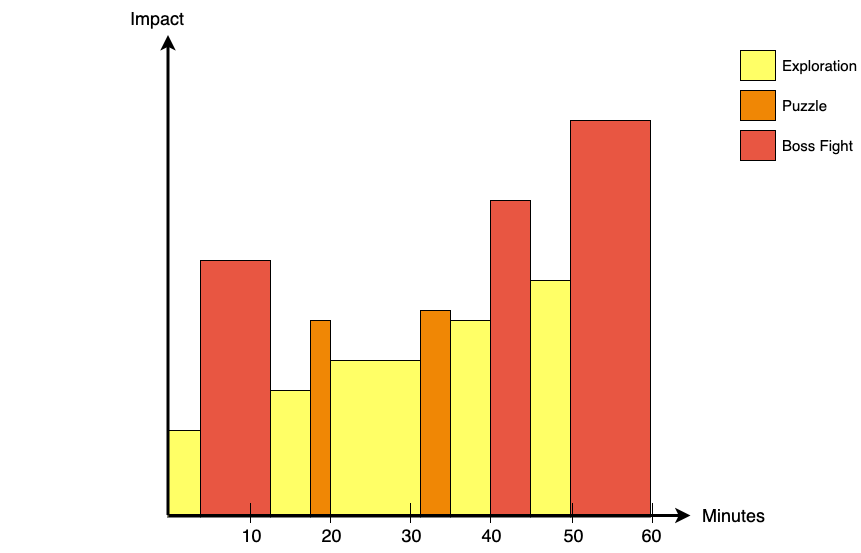
\includegraphics[width=0.8\linewidth]{images/graphs/event_diagram.png}
\end{figure}

\subsection{Level Map}

\begin{figure}[H]
	\centering
	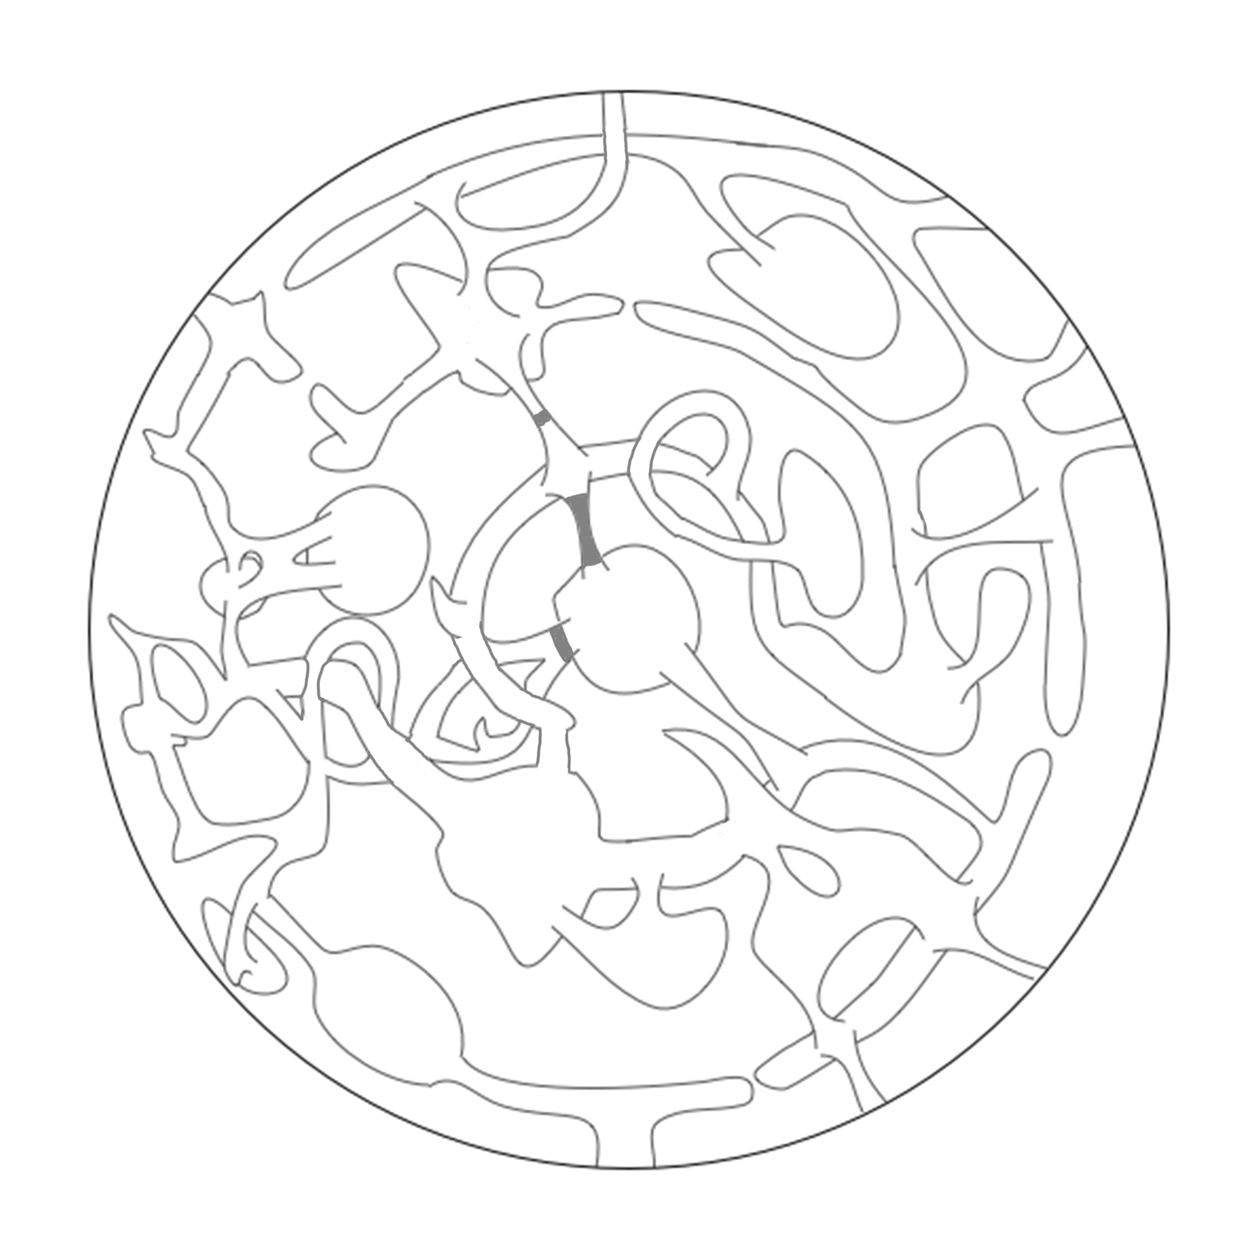
\includegraphics[width=0.6\linewidth]{images/map/map_clear.png}
	\caption*{Complete 2D map of the level}
\end{figure}

\begin{figure}[H]
	\centering
	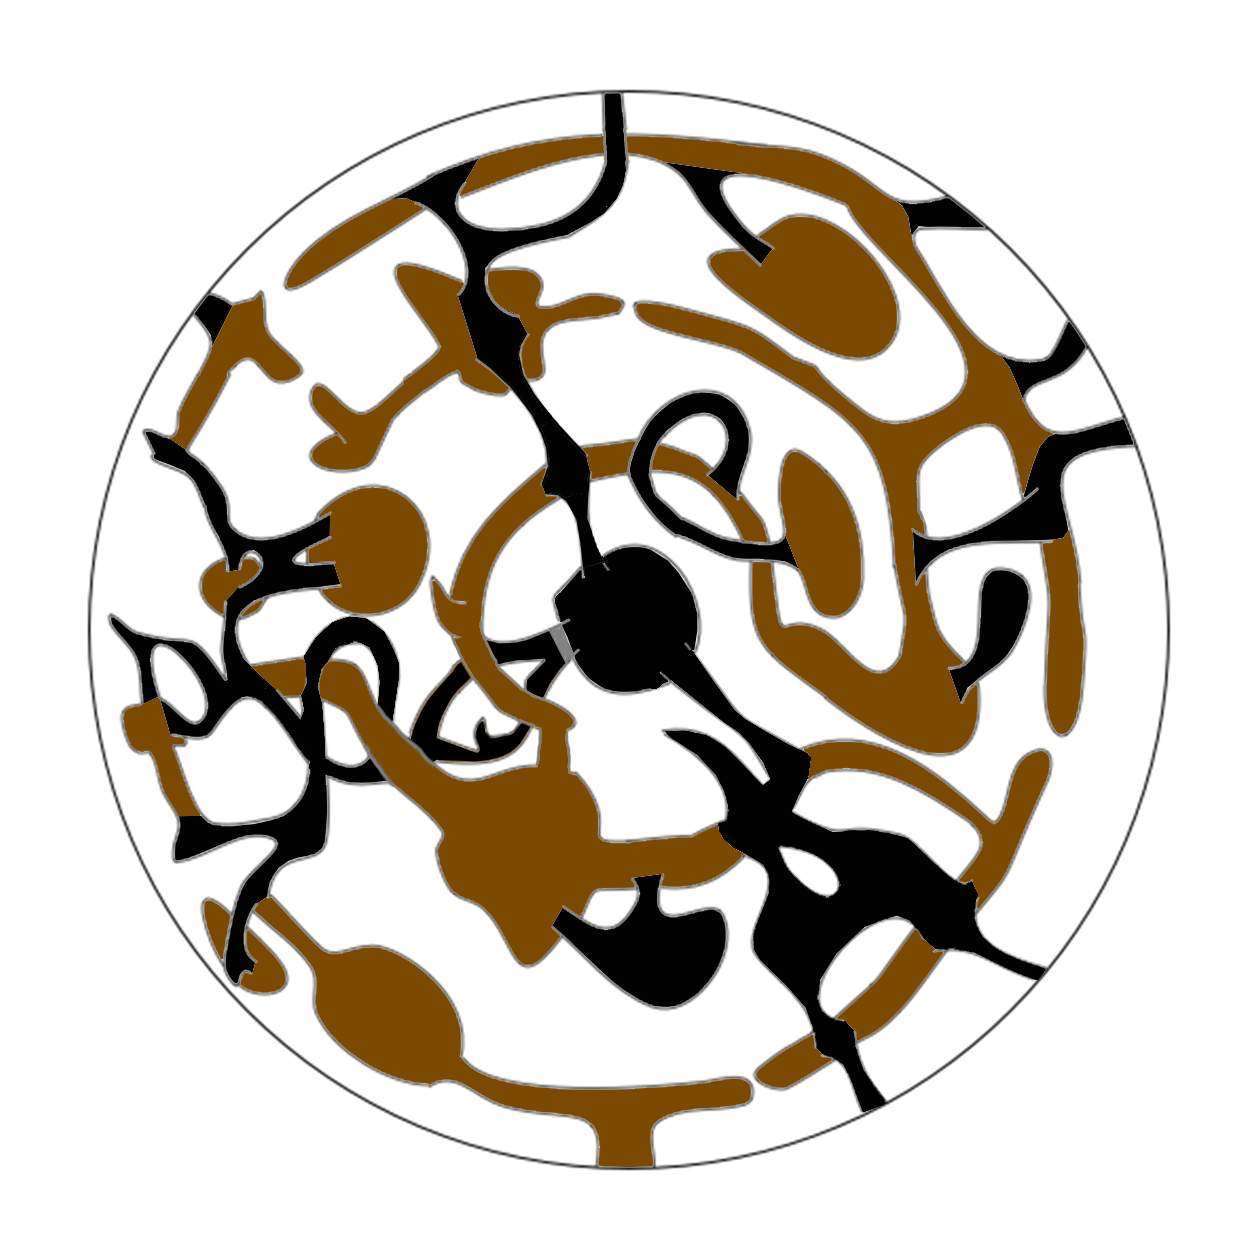
\includegraphics[width=0.6\linewidth]{images/map/2D_map_color.png}
	\caption*{Brown = Ground, Black = Vines}
\end{figure}

\begin{figure}[H]
	\centering
	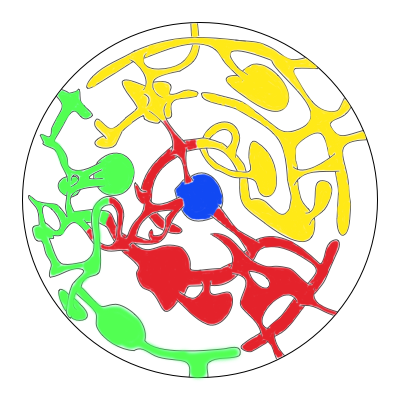
\includegraphics[width=0.6\linewidth]{images/map/map_all_sections.png}
	\caption*{Section 1: green, Section 2: yellow, Section 3: red, Boss Room: blue}
\end{figure}

\begin{figure}[H]
	\centering
	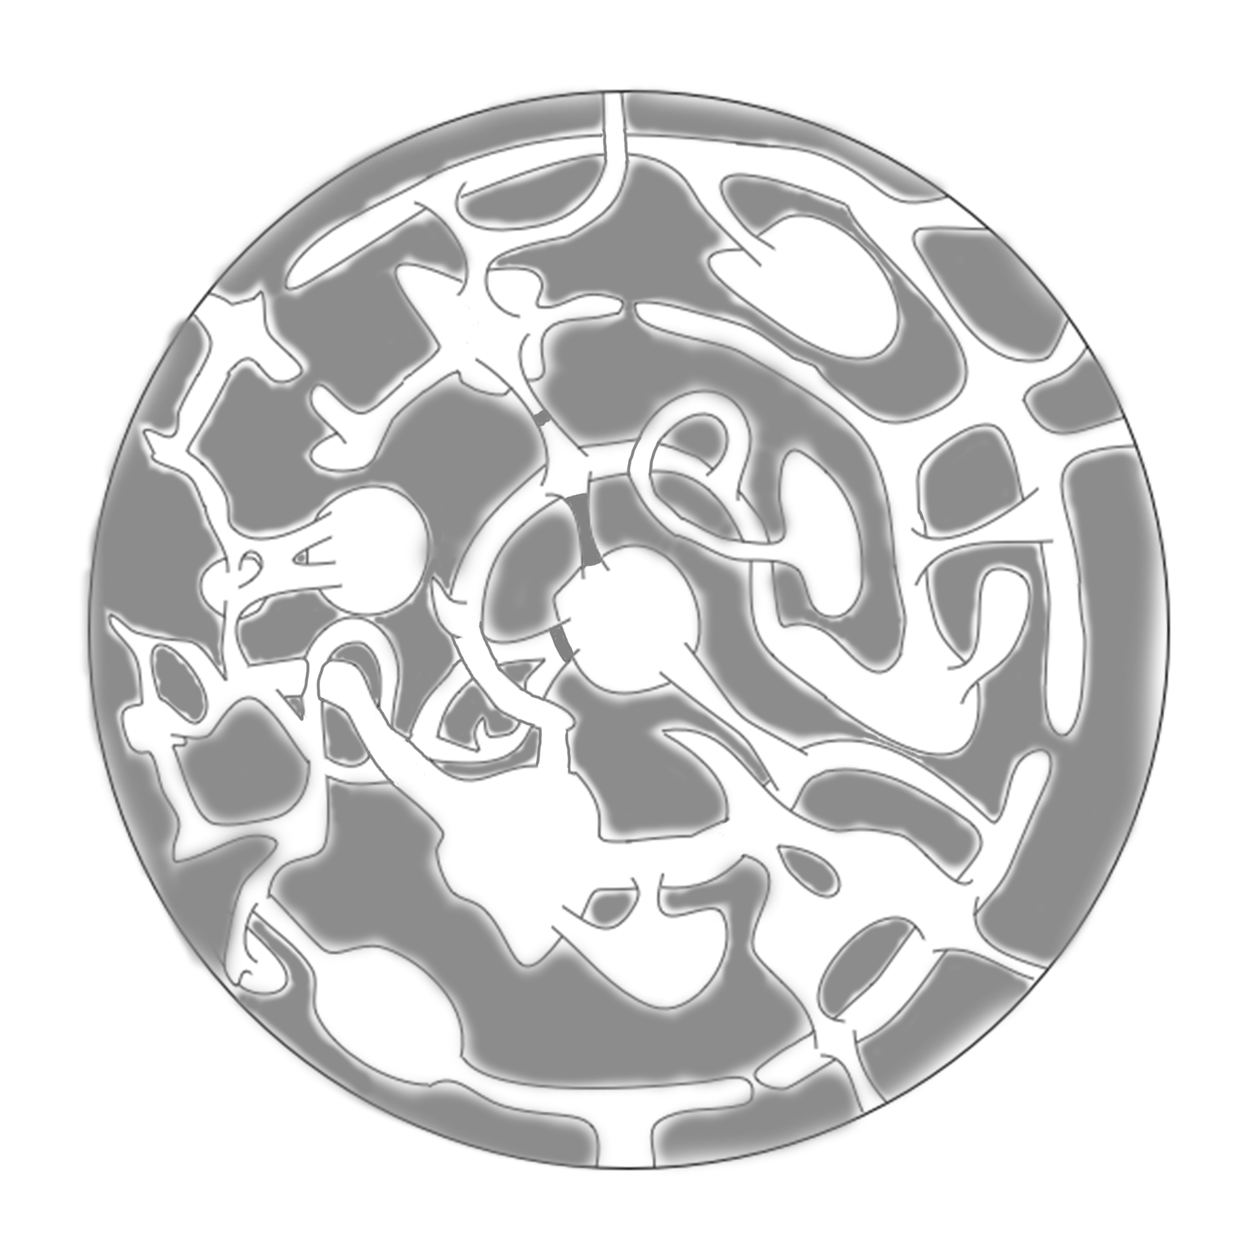
\includegraphics[width=0.6\linewidth]{images/map/2D_map_not.png}
	\caption*{Gray areas cannot be walked on by the player}
\end{figure}
\newpage

\subsubsection{Measures}
\begin{figure}[H]
	\centering
	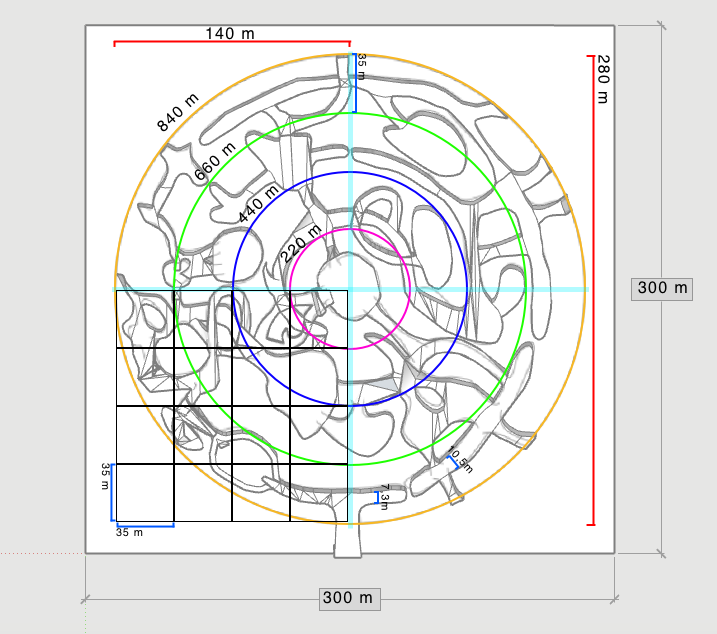
\includegraphics[width=14cm]{images/map/map_measures.png}
\end{figure}

\begin{figure}[H]
	\centering
	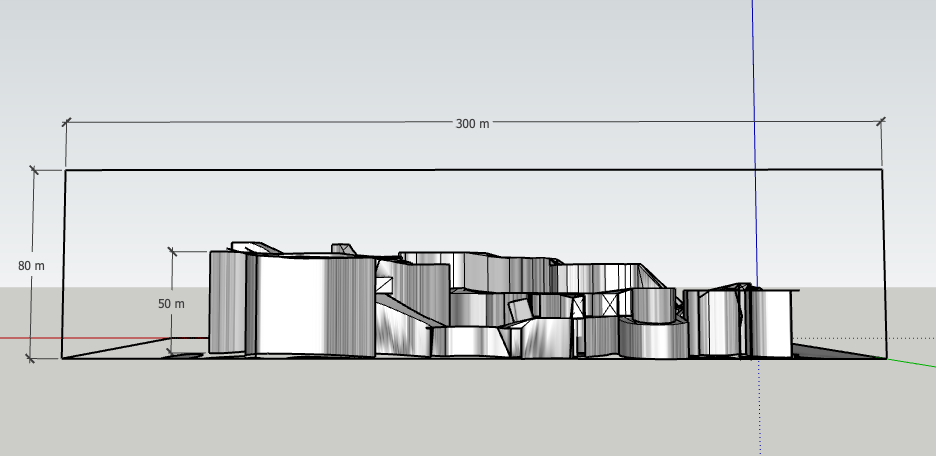
\includegraphics[width=14cm]{images/map/3D_map_half.png}
\end{figure}
\newpage

\subsection{Level Diagram}\label{legend}
\begin{figure}[H]
	\centering
	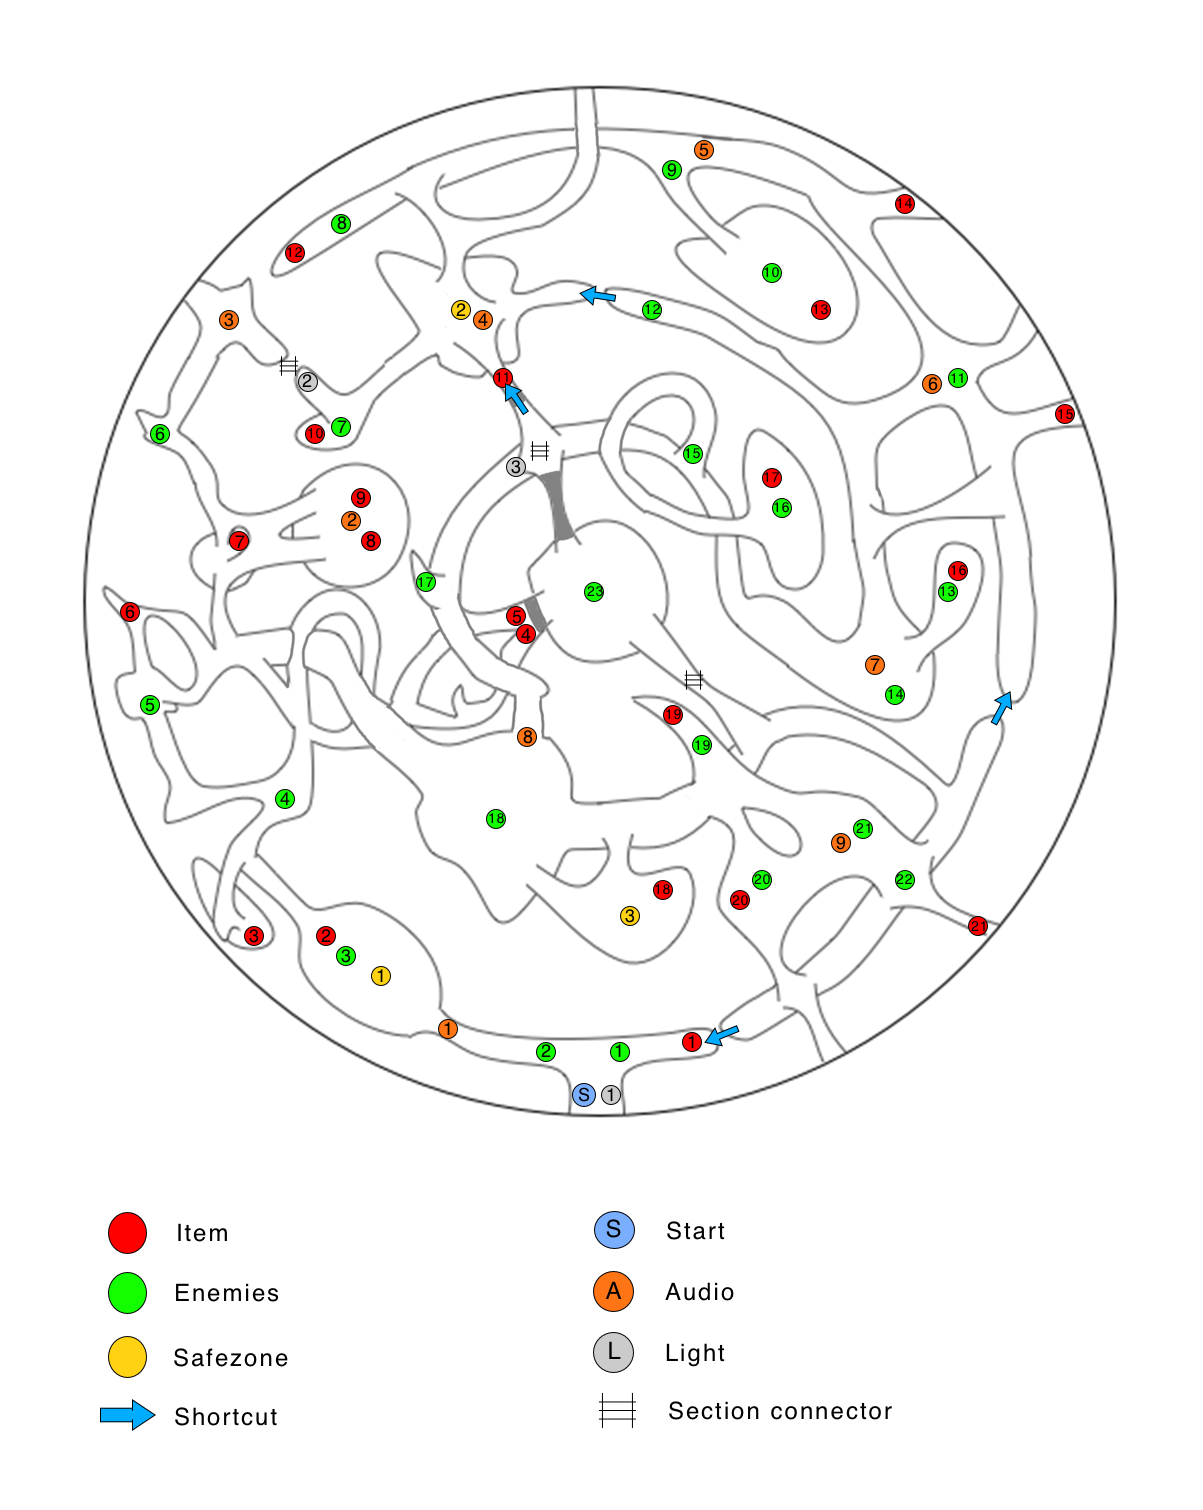
\includegraphics[width=0.95\linewidth]{images/map/map_legend.png}
\end{figure}
\newpage

\subsection{Level Description}
\begin{figure}[H]
	\centering
	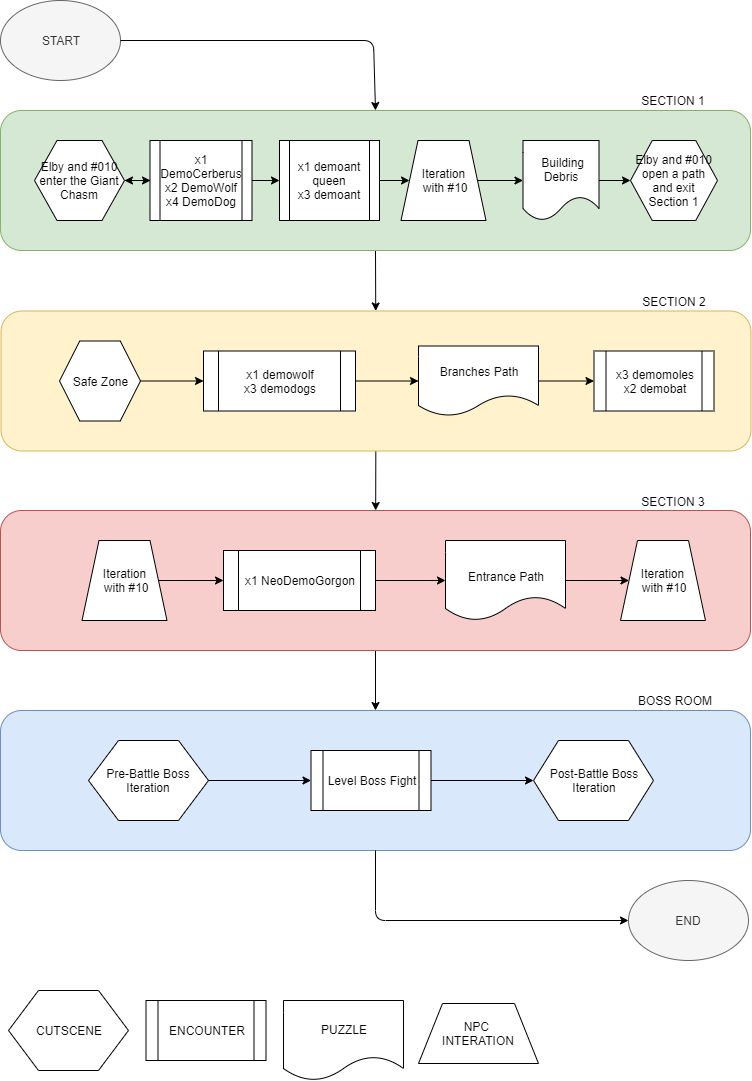
\includegraphics[width=0.95\linewidth]{images/graphs/level_description.png}
\end{figure}
\newpage


\subsubsection{Giant Chasm - Outside}
The level designed is the subarea 15 of the Core Enviroment. It is located in the north side of the City Ruins. The diameter of the giant chasm is at least 300m and its origins are unknown, even if in-game characters often assume that it originated from the impact of a meteorite. From the outside it is impossible to see the contents of the chasm due to the lack of internal light and for the thick crop of vines that surround the entire area. Fixed enemies are placed inside the rooms, while some monsters can randomly spawn along the way.

\begin{figure}[H]
	\centering
	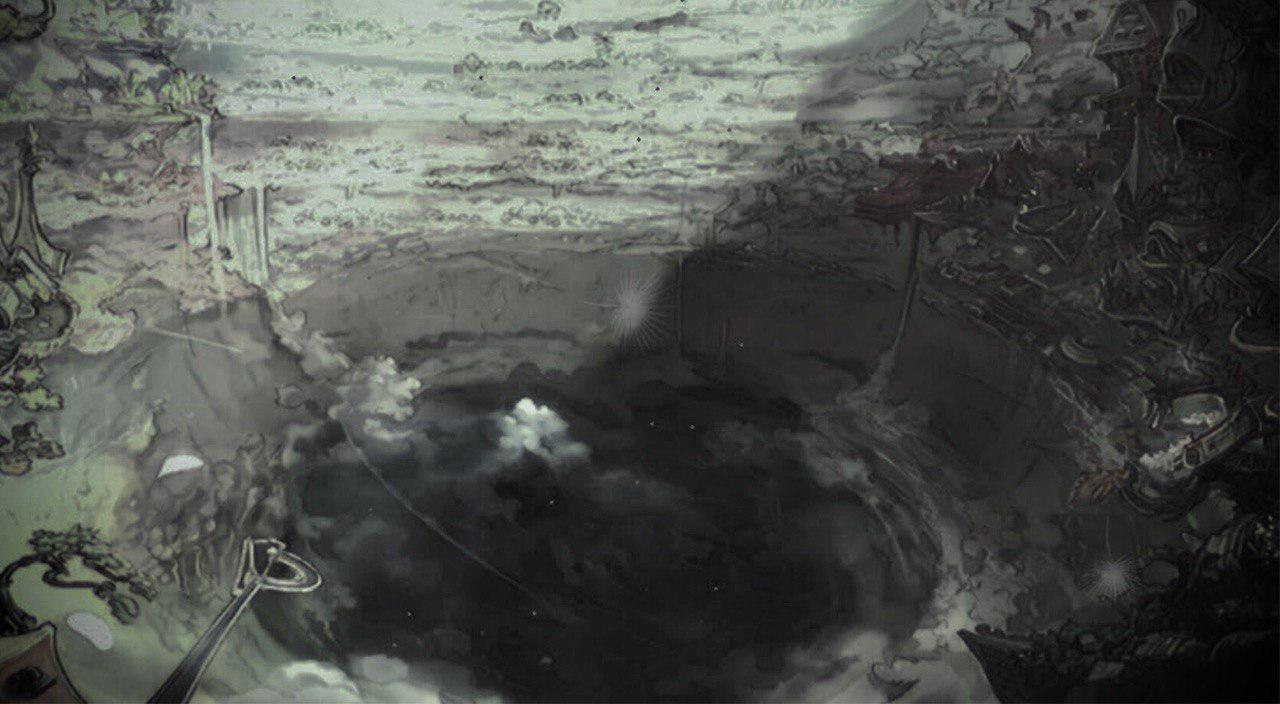
\includegraphics[width=0.8\linewidth]{images/visual_ref/15_giant_chasm/chasm_outside.jpg}
	\caption*{Overview of the Giant Chasm. \textit{[Made in the Abyss]}}
\end{figure}
\newpage


\subsubsection{Giant Chasm - Section 1}
The first section is approximately 500m long and with a variable width depending on the type of terrain (land, vines, etc.). Players enter through a gap in the south side of the Giant Chasm. The left side of the path is blocked by vines and debris and players can only unlock it from the other side in Section 3. Proceeding to the right, players reach the ballroom, where the DemoCerberus stands guard. After the first ruin, players will be forced to continue on the big vines coming from the lower levels of the Chasm, until they returns to the ridge. At the point of descent for the Second Section, it will be necessary to explore the surroundings in order to find a way to break through the obstacle.

\vspace*{0.3cm}
\begin{figure}[H]
	\centering
	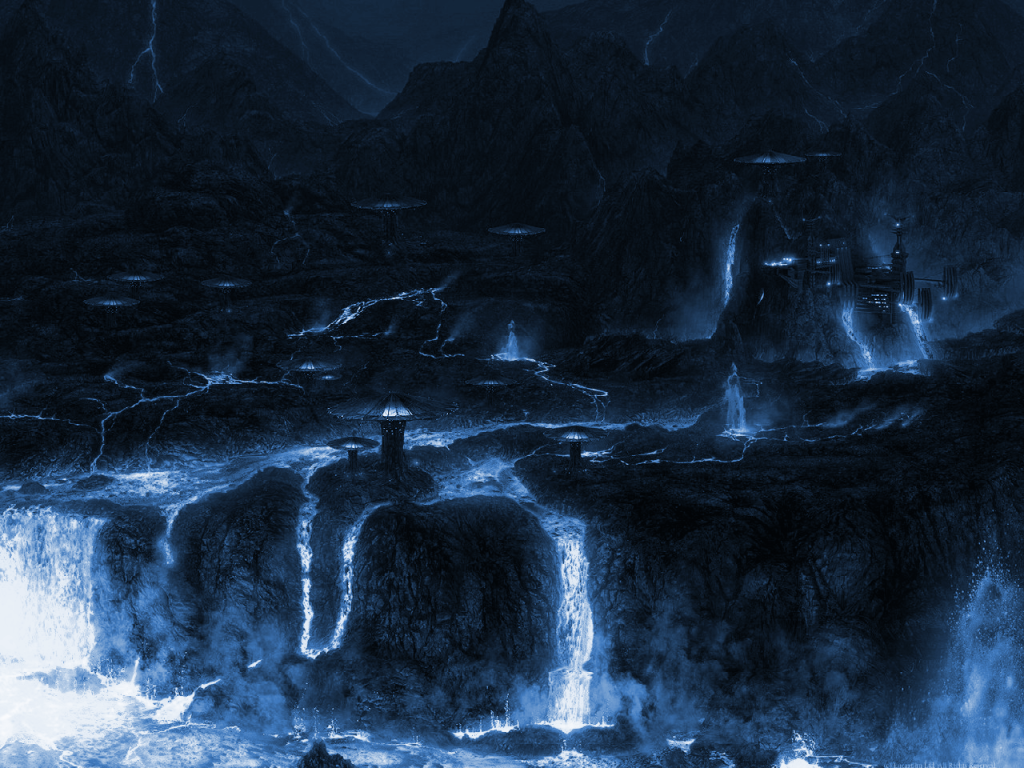
\includegraphics[width=0.7\linewidth]{images/visual_ref/15_giant_chasm/chasm_section_1.png}
	\caption*{Path of the first section}
\end{figure}

\begin{figure}[H]
	\centering
	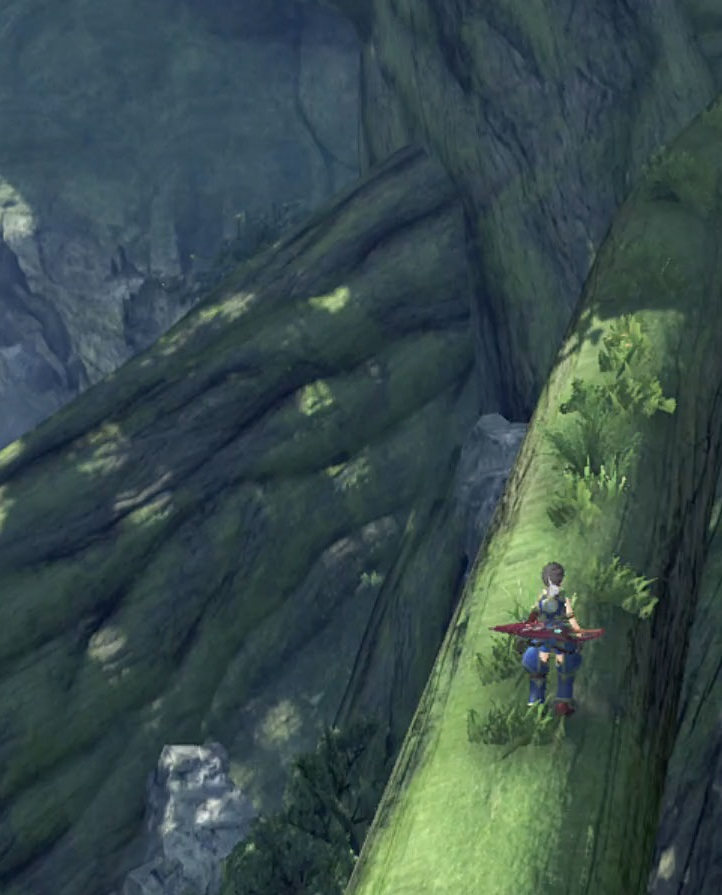
\includegraphics[width=0.5\linewidth]{images/visual_ref/15_giant_chasm/tree.jpg}
	\caption*{Visual example of the player walking on a vine}
\end{figure}

\begin{figure}[H]
	\centering
	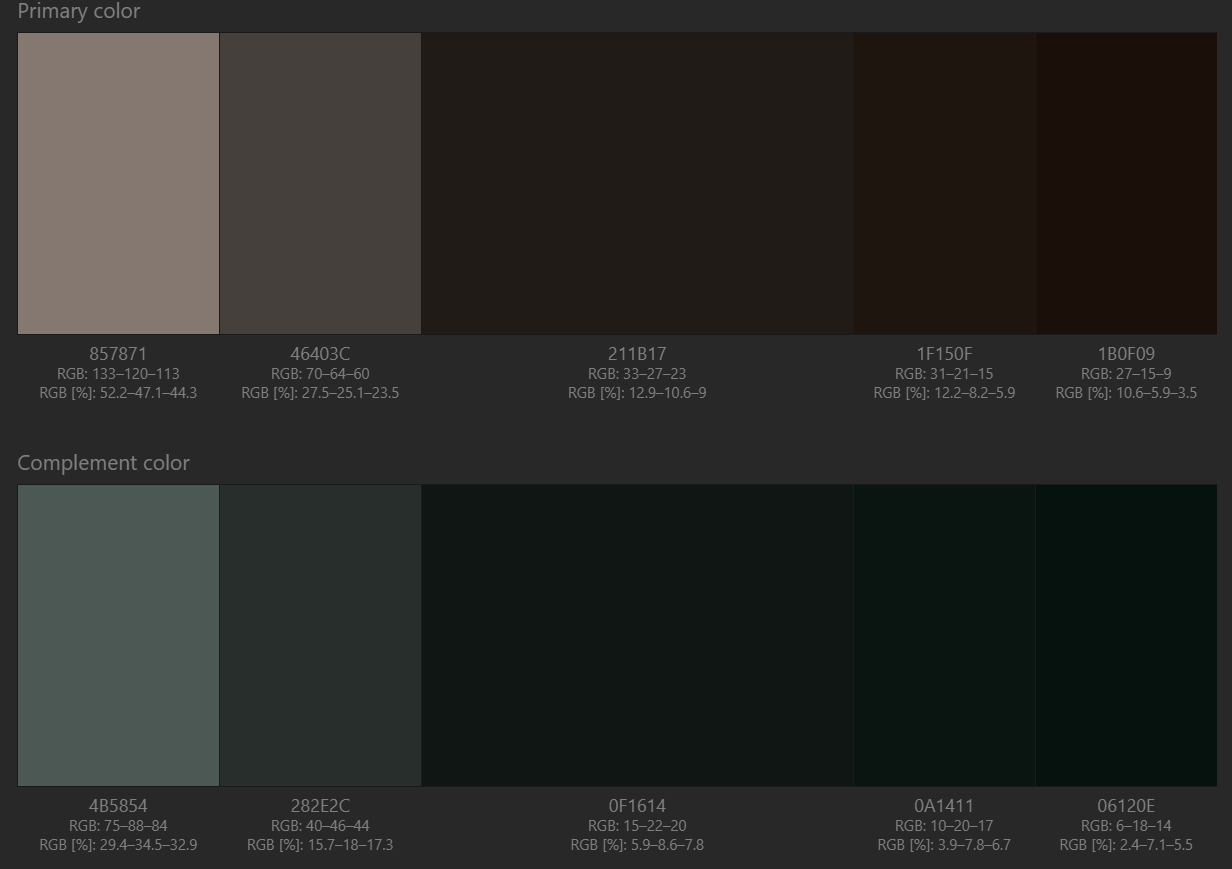
\includegraphics[width=0.8\linewidth]{images/visual_ref/15_giant_chasm/pallette/pallette_section_01.png}
	\caption*{Primary color = ground, secondary color = vines}
\end{figure}

\begin{figure}[H]
	\centering
	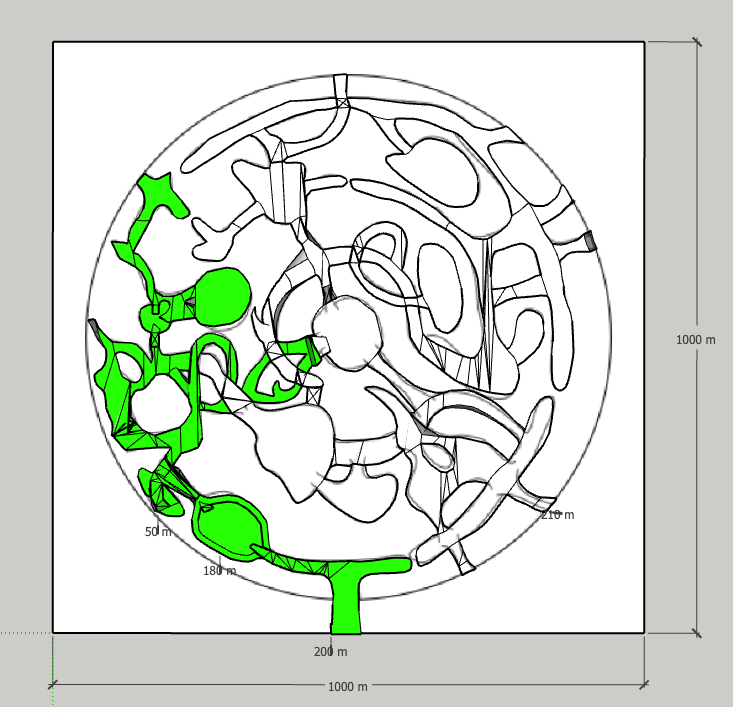
\includegraphics[width=0.7\linewidth]{images/map/2D_map_section_01.png}
	\caption*{Section 1}
\end{figure}

\begin{figure}[H]
	\centering
	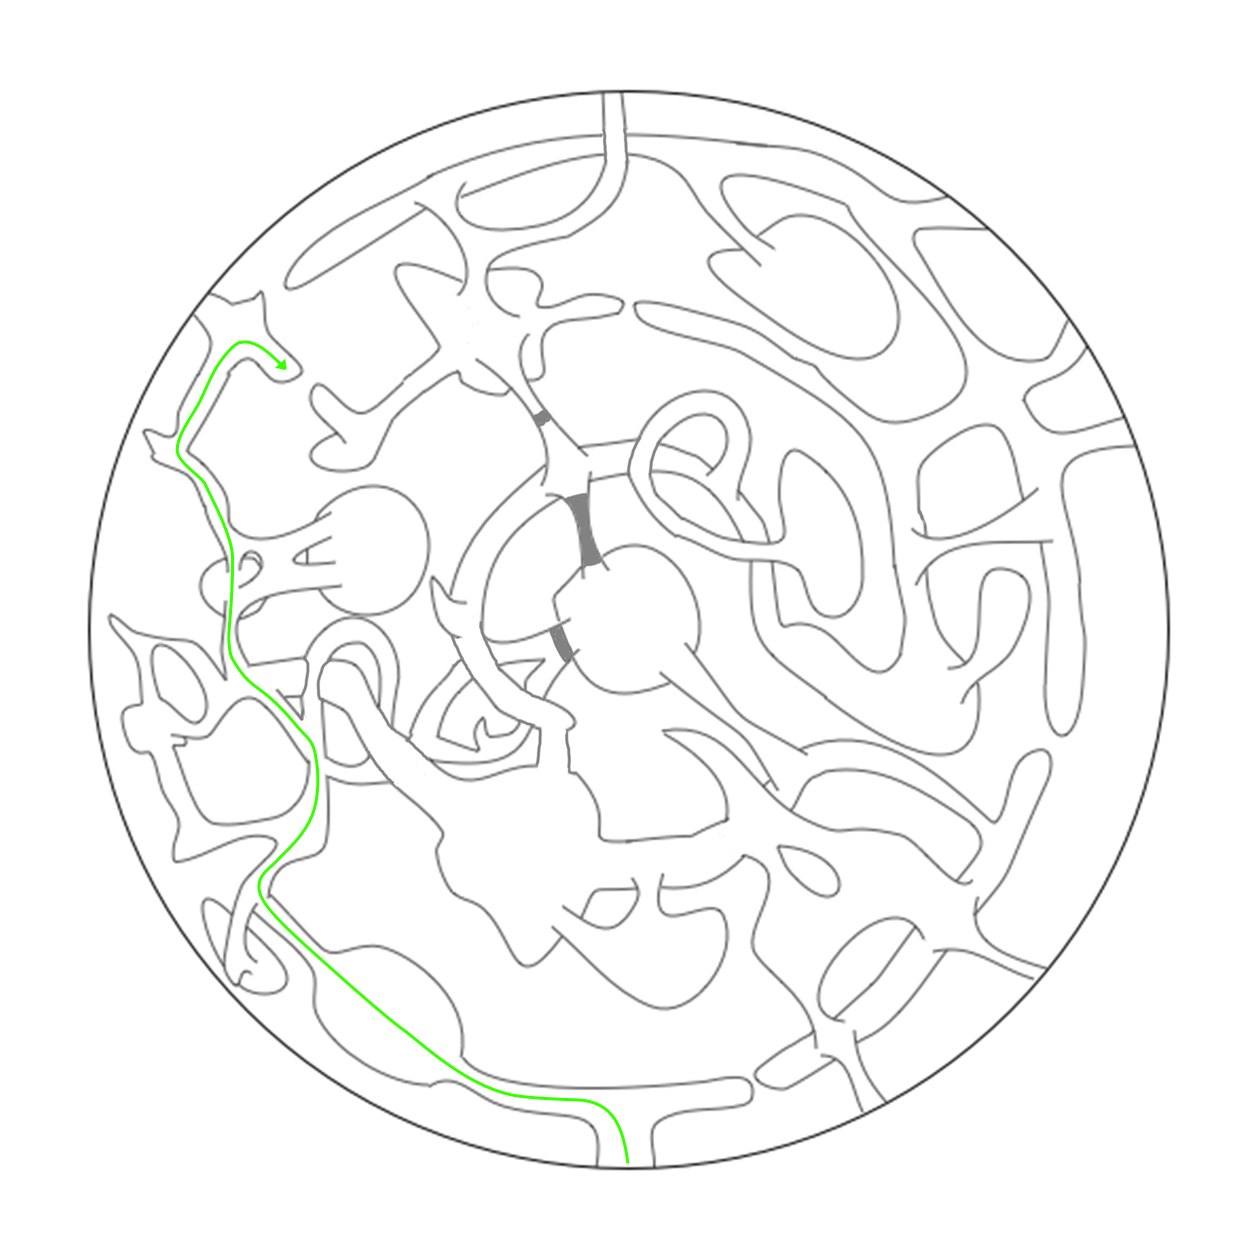
\includegraphics[width=0.7\linewidth]{images/map/map_principle_path_section_01.png}
	\caption*{Section 1 main path}
\end{figure}

\textbf{Encounters}
\begin{itemize}
	\item 1x DemoCerberus
	\item 2x DemoWolf
	\item 4x DemoDog
\end{itemize}
The Democerberus is considered a mini-boss and its statistics are proportionally reduced compared to its previous Level Boss version. At the entrance to the room, the DemoCerberus, previously in a resting position, enters an offensive state, remaining however to guard the exit of the ruin. Once the first damage threshold has been exceeded, the monster will recall two DemoWolves, which will immediately attack the players. Until the DemoWolves are defeated, the DemoCerberus will not attack and will be invulnerable. Ultimatly, upon reaching the second threshold, the Democerberus will call up four DemoDogs and it will apply the previous pattern.

\begin{itemize}
	\item 1 - 50\% Demorat, 30\% Demobat, 20\% Demodog
	\item 2 - 15\% Demowolves, 35\% Demobat, 50\% Demodog
	\item 3 - Democerberus x1
	\item 4 - 50\% Demorat, 30\% Demobat, 20\% Demodog
	\item 5 - 50\% Demorat, 30\% Demobat, 20\% Demomoles
	\item 6 - 20\% Demomoles, 60\% Demobat, 20\% Demodog
\end{itemize}

*Map points on chapter \ref{legend}.\\

\textbf{Sounds}\\
DemoDog / DemoWolf howls can be heard randomly. Near the ruins there is a sound of landslides. The sound of Elby's footsteps changes according to the terrain on which she is located.

\begin{itemize}
	\item 1 - Howling wolves
	\item 2 - Moaning monsters
	\item 3 - Landslide noise
\end{itemize}

*Map points on chapter \ref{legend}.\\

\textbf{Lighting}\\
There's a soft white light coming from the few opening in the crop of vines. It is also possible to see a slight red light coming from the chasm center. The rooms in the ruins are illuminated by a strange luminous moss.

\begin{itemize}
	\item 1 - Trigger light change
\end{itemize}

*Map point on chapter \ref{legend}.\\

\textbf{Drops}
\begin{itemize}
	\item 1 - Fresh moss
	\item 2 - Rooten potion
	\item 3 - Rotten root
	\item 4 - Demowolf Tooth
	\item 5 - Fresh root
	\item 6 - Rotten moss
	\item 7 - Rotten moss
	\item 8 - Fresh elisir
	\item 9 - Demorat Tail
\end{itemize}

*Map points on chapter \ref{legend}.\\

\textbf{Puzzle}\\
To change area Elby will find herself facing a bridge of dry and weak vines. At this point, in order to be able to move on, she will need to freeze the vines so as to strengthen them.\\
The path melts very quickly so that the protagonist can only cross each box once. once all the quadrants are weakened, the block will break making it fall. Elby will therefore have to be at the point indicated by the X in the image below in order to continue his journey. If this does not happen, \#010 will repeat the reconstruction of the bridge to prevent it from falling and injuring Elby. The latter will lose a quarter of its life and will have to repeat the operation.\\
The path can be solved as follows:\\

\textit{Main Solution}\\
up / left x2 / up x4 / right / down x3 / right x2 / down / right / up x4 / left / down x2 / left / up x2\\

\begin{figure}[H]
	\centering
	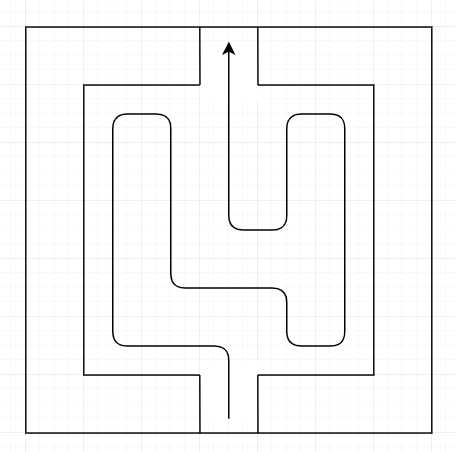
\includegraphics[width=0.5\linewidth]{images/puzzle/puzzle_011.png}
\end{figure}

\textit{Alternative Solution}\\
up / left x2 / up x2 / right / down / right x2 / down / right / up x4 / left / down x2 / left / up / left x2 / up / right x2 / up\\

\begin{figure}[H]
	\centering
	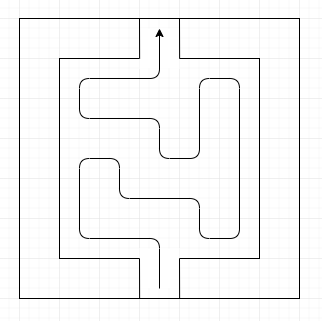
\includegraphics[width=0.5\linewidth]{images/puzzle/puzzle_012.png}
\end{figure}
\newpage


\subsubsection{Giant Chasm - Section 2}
The second section is about 600m long and takes players to the first underground layer.
Compared to Section 1, the route is narrower and made up of tunnels that allow you to move upwards or downwards and reach platforms and / or ridges that cannot be accessed in other ways. Players will often be asked to use skills to open passages and / or move debris. The soil, where it is not covered with organic vines, is very irregular due to the proximity of the nucleus and the presence of many DemoMoles. Players will find a Safe Room near the beginning of Section 2, and they will unlock a path to reach the room again just before Section 3.

\vspace*{0.3cm}
\begin{figure}[H]
	\centering
	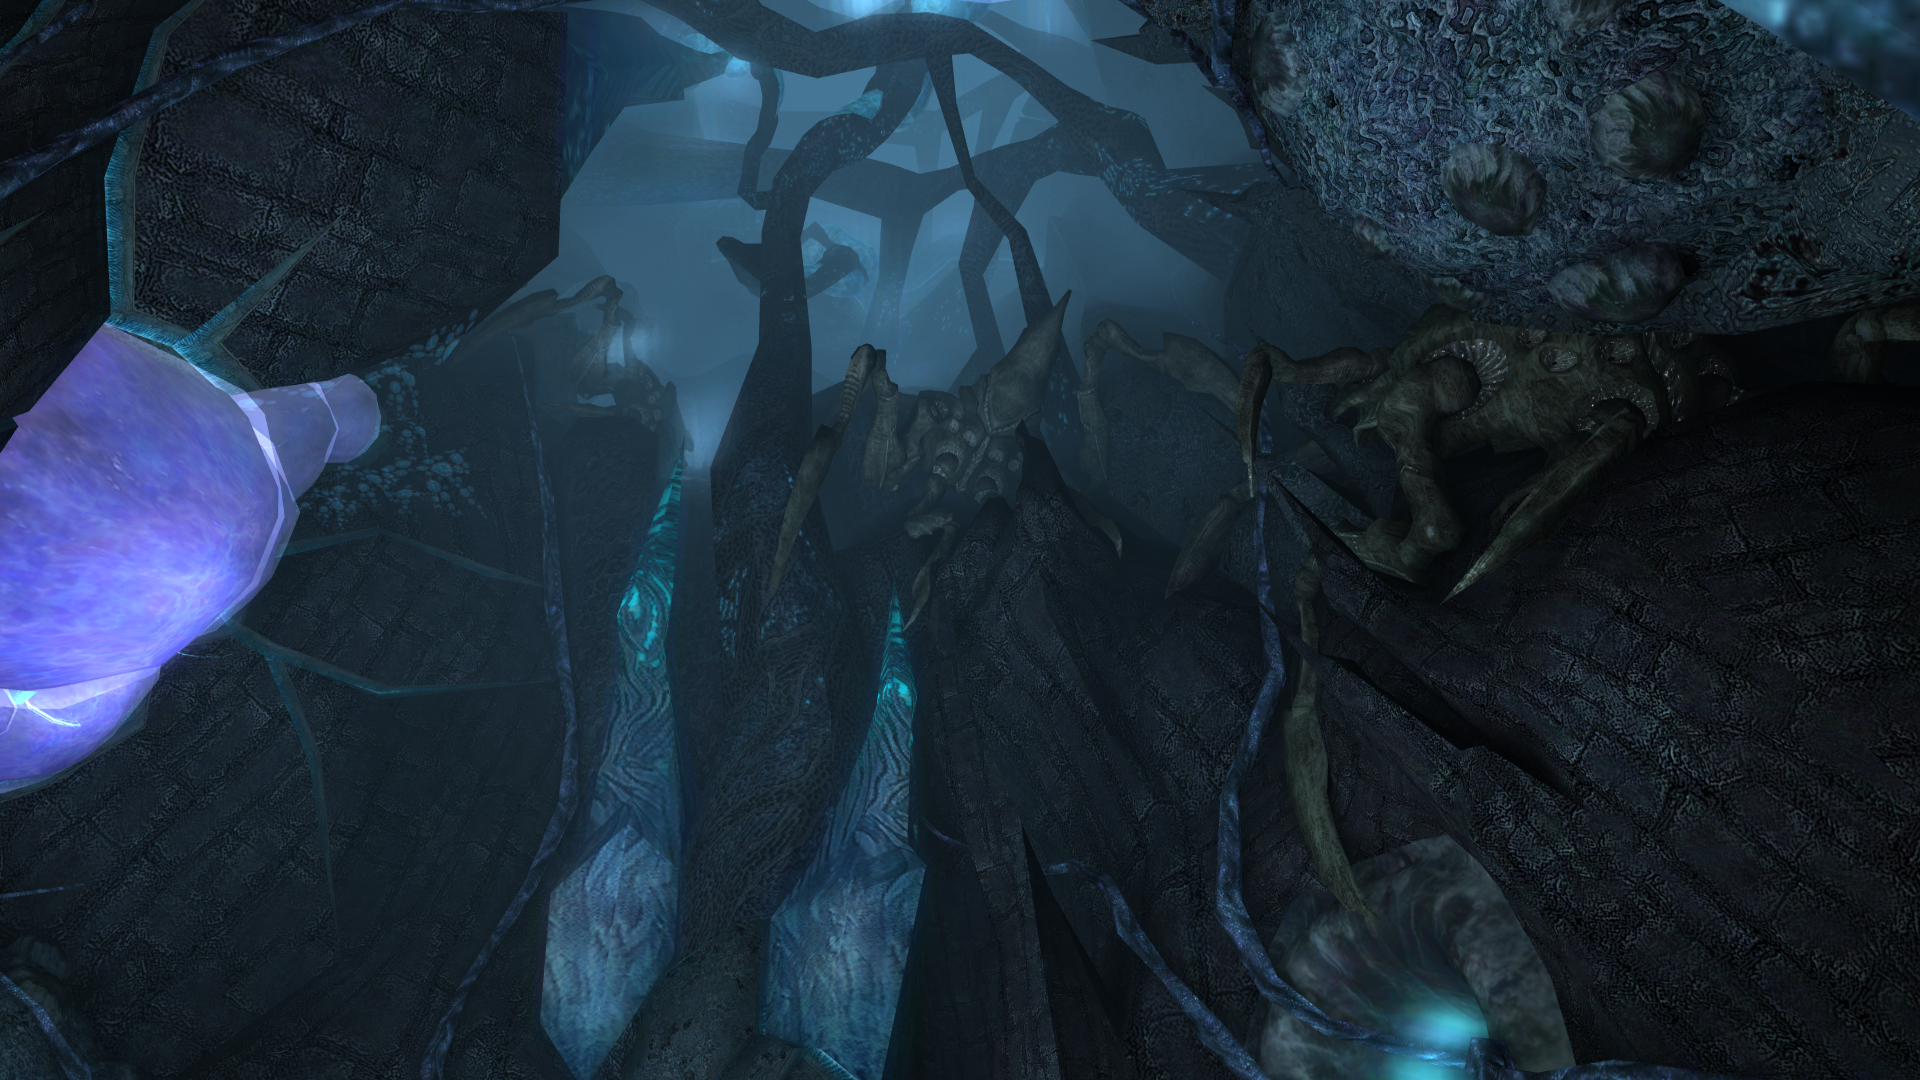
\includegraphics[width=0.8\linewidth]{images/visual_ref/15_giant_chasm/chasm_section_2.png}
	\caption*{Path of the second section}
\end{figure}

\begin{figure}[H]
	\centering
	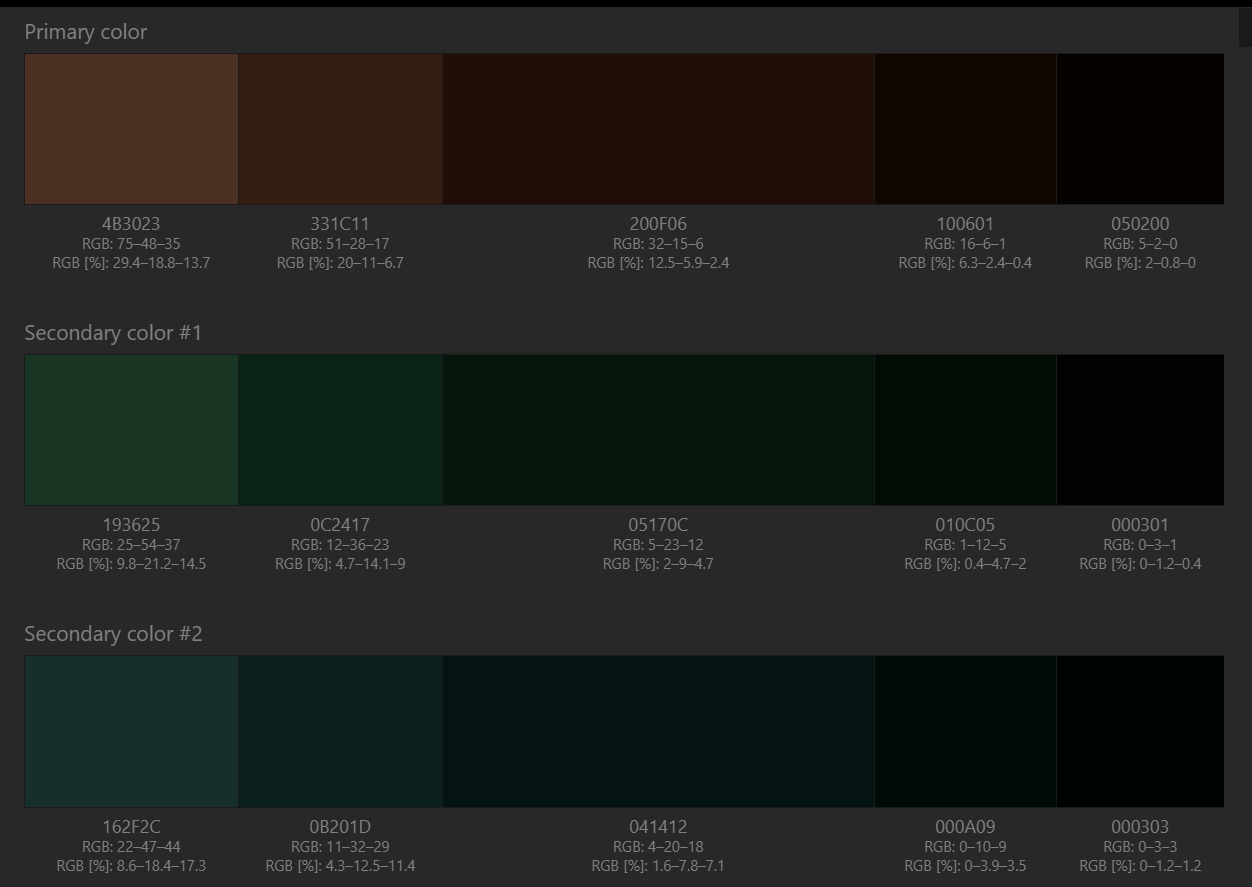
\includegraphics[width=0.8\linewidth]{images/visual_ref/15_giant_chasm/pallette/pallette_section_02.png}
	\caption*{Primary color = ground, secondary color = vines}
\end{figure}

\begin{figure}[H]
	\centering
	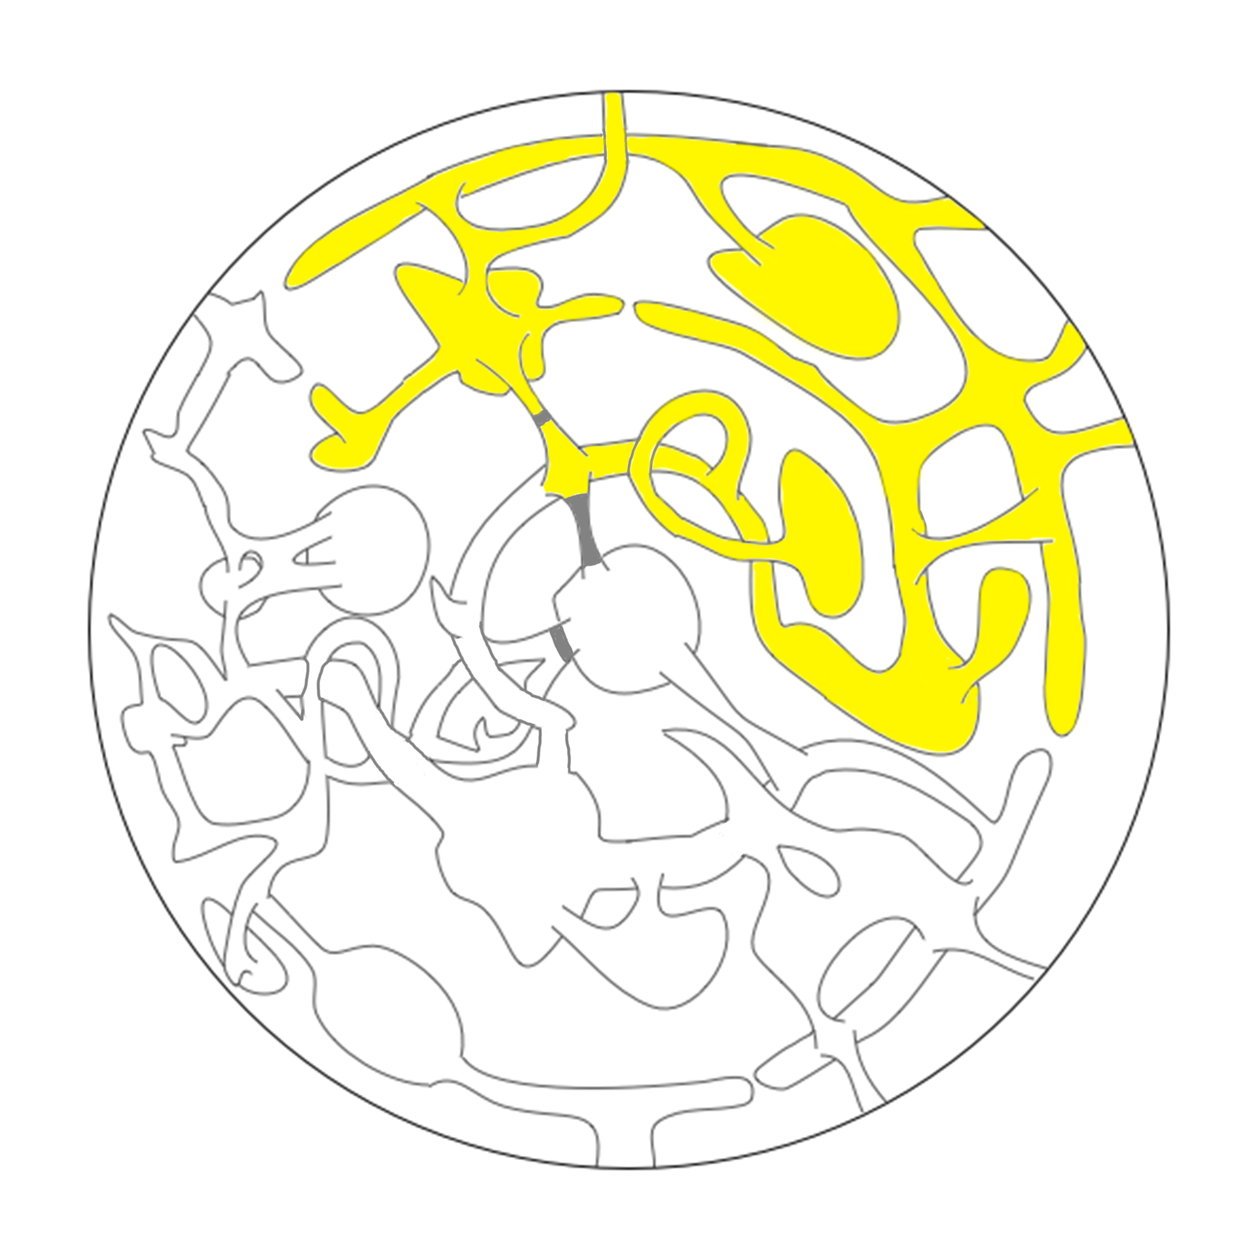
\includegraphics[width=0.7\linewidth]{images/map/2D_map_section_02.png}
	\caption*{Section 2}
\end{figure}

\begin{figure}[H]
	\centering
	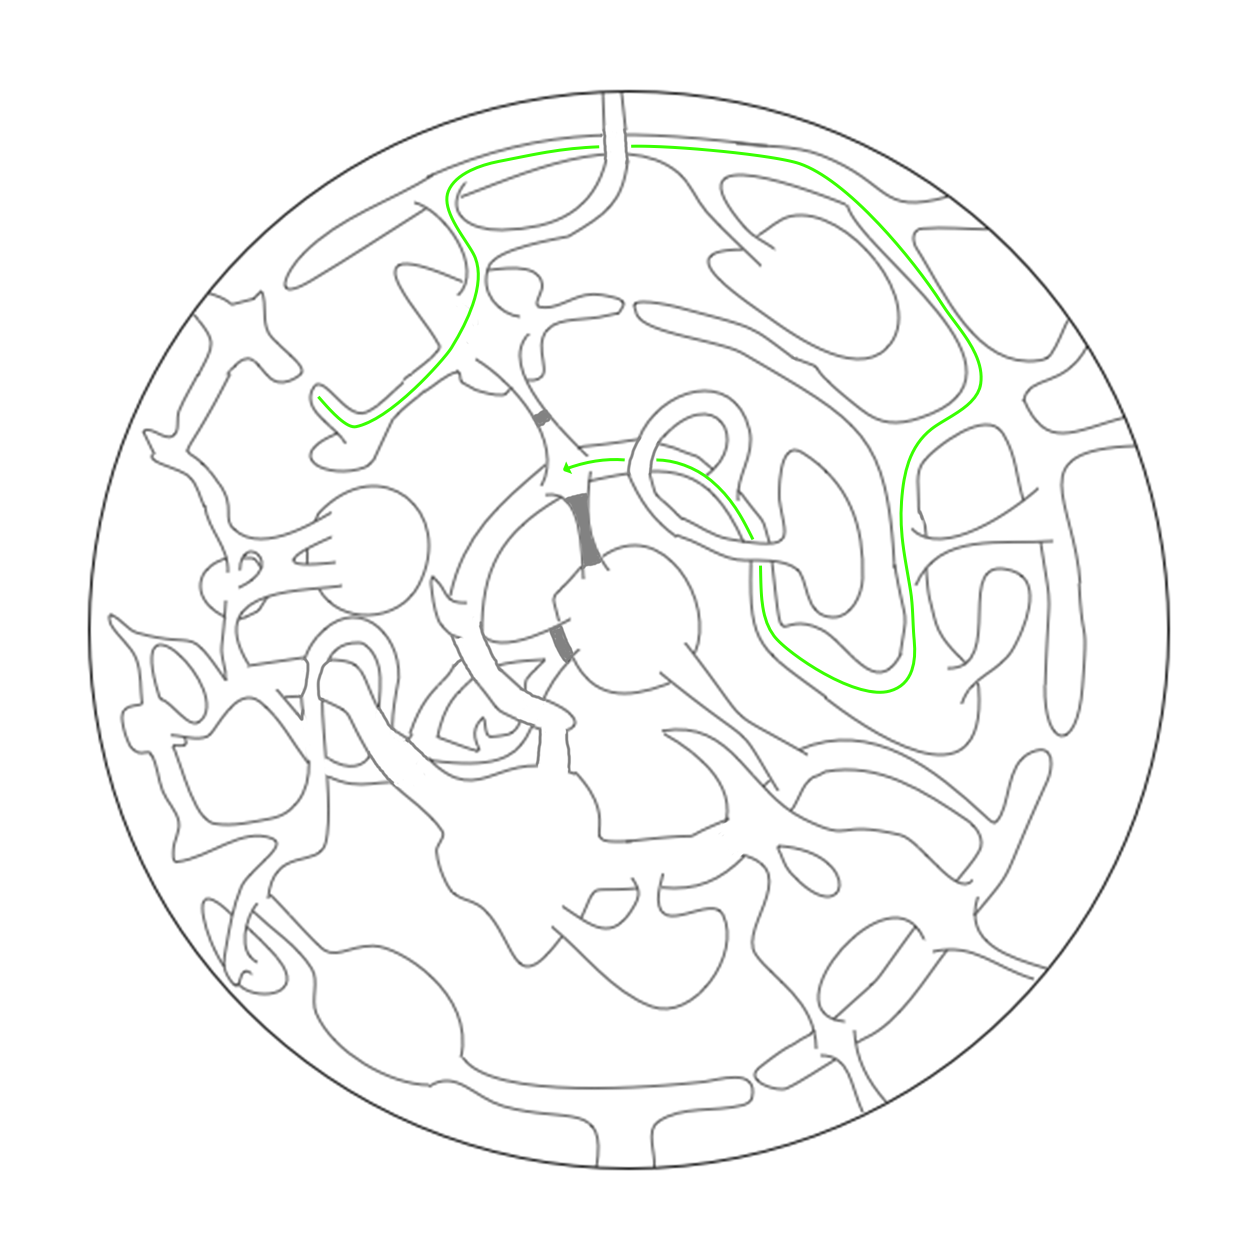
\includegraphics[width=0.7\linewidth]{images/map/map_principle_path_section_02.png}
	\caption*{Section 2 main path}
\end{figure}

\textbf{Encounter A}
\begin{itemize}
	\item x1 DemoWolf
	\item x2 DemoDog
\end{itemize}
A herd of DemoWolf. Players can kill DemoDogs one at a time to deal individually with the DemoWolf. Otherwise, if the DemoWolf is alerted, it will trigger all the DemoDogs in the room.\\

\textbf{Encounter B}
\begin{itemize}
	\item x2 DemoMoles
	\item x1 DemoBat
\end{itemize}
Entering the ruin, the player will find it empty. Once in the middle of the room, Elby and \#010 will remain stuck in the ground, and the player will have a few seconds to activate the Levitation skill to avoid taking damage (Quick Time Event). Finally, the DemoMoles and DemoBats will appear, starting the battle.

\begin{itemize}
	\item 7 - 50\% Demorat, 30\% Demobat, 20\% Demodog
	\item 8 - 20\% Demorat, 60\% Demobat, 20\% Demodog
	\item 9 - 15\% Demowolves, 35\% Demobat, 50\% Demodog
	\item 10 - 50\% Demorat, 30\% Demobat, 20\% Demodog
	\item 11 - 20\% Demobat, 60\% Demorat, 20\% Demodog
	\item 12 - 50\% Demorat, 30\% Demobat, 20\% Demodog
	\item 13 - Demowolf x1, Demodog x2
	\item 14 - 20\% Demorat, 60\% Demobat, 20\% Demodog
	\item 15 - 40\% Demorat, 40\% Demobat, 20\% Demomoles
	\item 16 - Demomoles x2, Demobat x1
\end{itemize}


\textbf{Sounds}\\
The rustling of moving vines can be heard randomly. The sound of Elby's footsteps changes according to the terrain on which she is located.

\begin{itemize}
	\item 4 - Landslide
	\item 5 - Flapping of wings
	\item 6 - Whoosh vines
	\item 7 - Landslide
\end{itemize}

\textbf{Lighting}\\
There's no light coming from above. The only lights are the white one coming from the moss and the red one coming from the core (more intense than Section 1).

\begin{itemize}
	\item 2 - Trigger light change
\end{itemize}

\newpage

\textbf{Drops}
\begin{itemize}
	\item 10 - Rotten elisir
	\item 11 - Monster meat
	\item 12 - Demorat Tail
	\item 13 - Fresh root
	\item 14 - Demowolf Tooth
	\item 15 - Rotten root
	\item 16 - Rotten moss
	\item 17 - Demorat Tail
\end{itemize}

\textbf{Puzzle}\\
Bad Eleven will find the street blocked by a lot of rocks. So she has to push them away, in the correct order, with his special mental ability. When there are no more moves available or the puzzle is irreversibly unsolvable, a dialogue line of \#010 will appear and then the room will be reset.
The path can be solved as follows:\\

\begin{figure}[H]
	\centering
	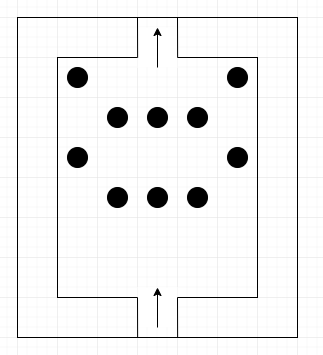
\includegraphics[width=0.7\linewidth]{images/puzzle/puzzle_021.png}
\end{figure}

\begin{figure}[H]
	\centering
	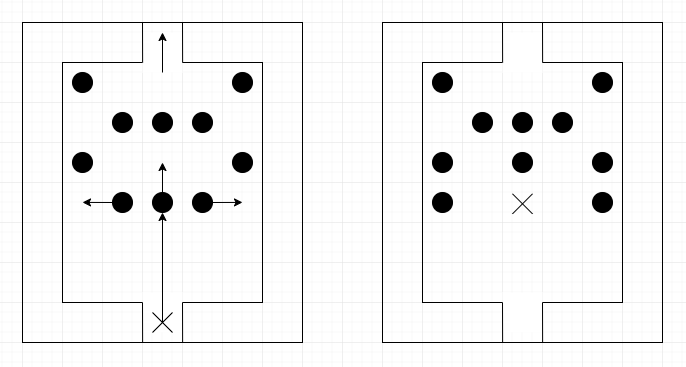
\includegraphics[width=0.8\linewidth]{images/puzzle/puzzle_022.png}
	\caption*{First step}
\end{figure}

\begin{figure}[H]
	\centering
	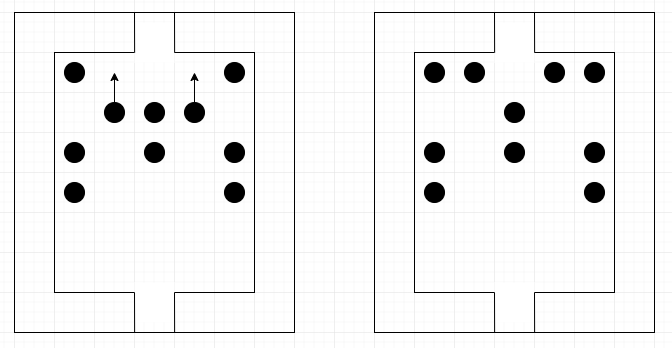
\includegraphics[width=0.8\linewidth]{images/puzzle/puzzle_023.png}
	\caption*{Second step}
\end{figure}

\begin{figure}[H]
	\centering
	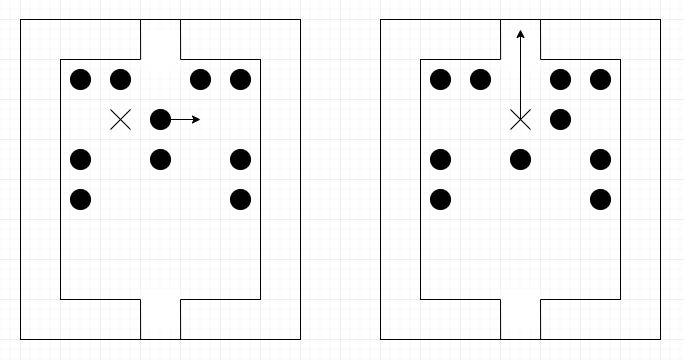
\includegraphics[width=0.8\linewidth]{images/puzzle/puzzle_024.png}
	\caption*{Third step}
\end{figure}
\newpage

\subsubsection{Giant Chasm - Section 3}
The third and final section is about 300m long and brings players to the second underground layer. It is not possible to follow any terrain course, forcing the players to climb and descend from the multitude of organic vines coming from the core, now extremely close. In this section players can explore the ramifications to obtain useful items and / or unlock the passage to the entrance of the abyss, allowing a possible backtracking. Following the main path and after facing the NeoDemoGorgon in his den, the player finally arrives in front of the gap for the heart of the Giant Chasm.

\vspace*{0.3cm}
\begin{figure}[H]
	\centering
	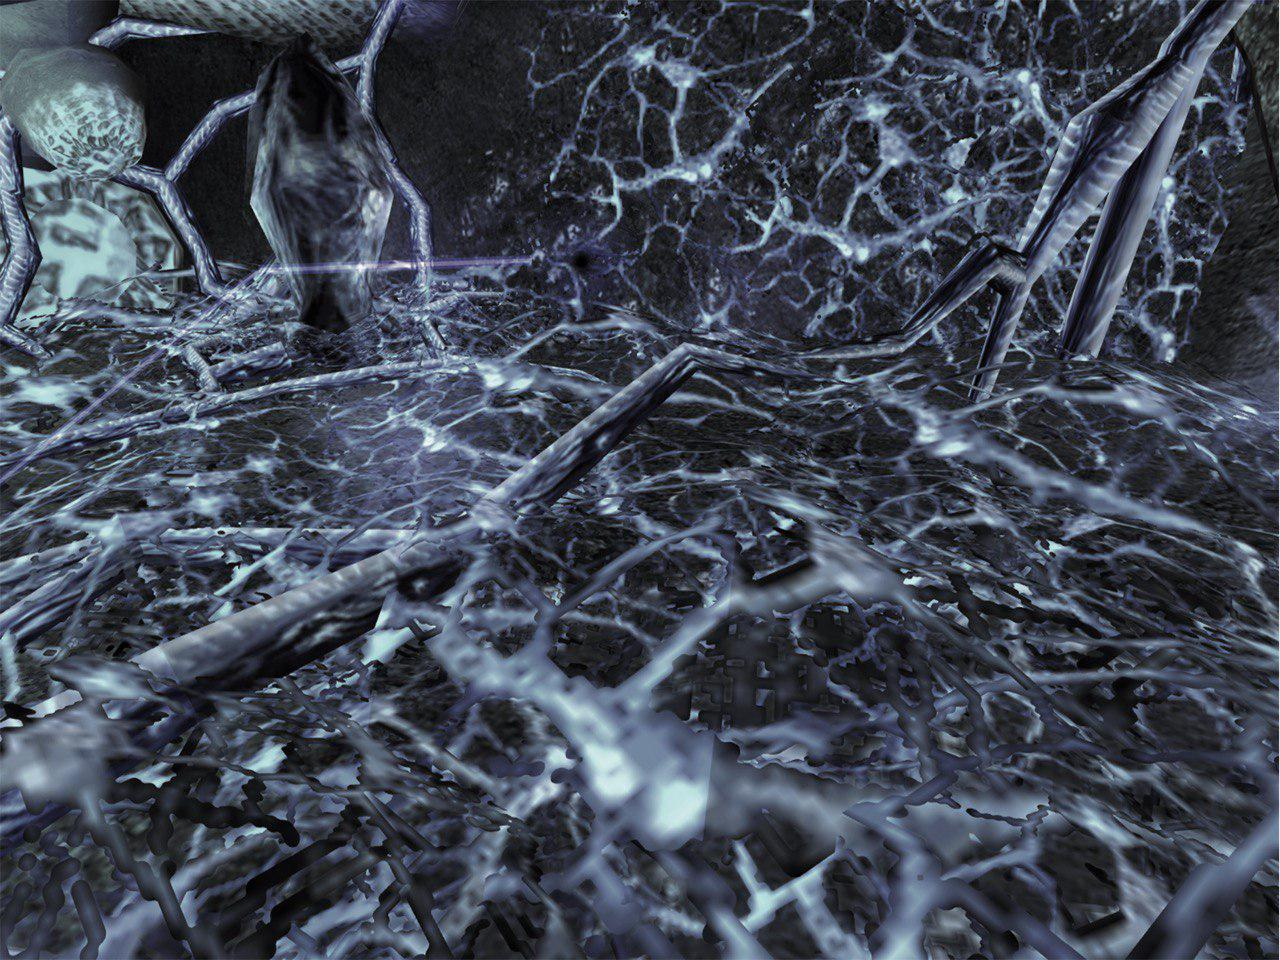
\includegraphics[width=0.8\linewidth]{images/visual_ref/15_giant_chasm/chasm_section_3.jpg}
	\caption*{Ground in the third section}
\end{figure}

\begin{figure}[H]
	\centering
	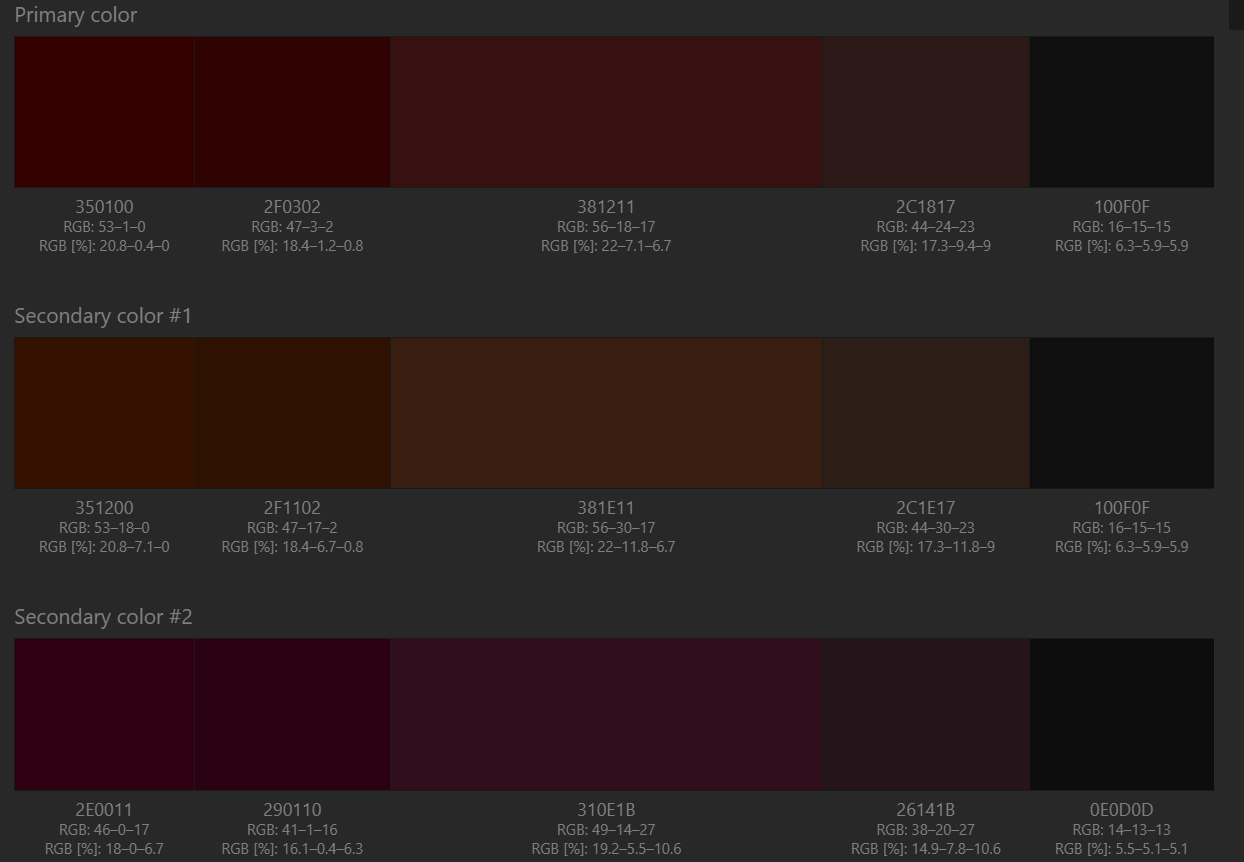
\includegraphics[width=0.8\linewidth]{images/visual_ref/15_giant_chasm/pallette/pallette_section_03.png}
	\caption*{Primary color = ground, secondary color = vines}
\end{figure}

\begin{figure}[H]
	\centering
	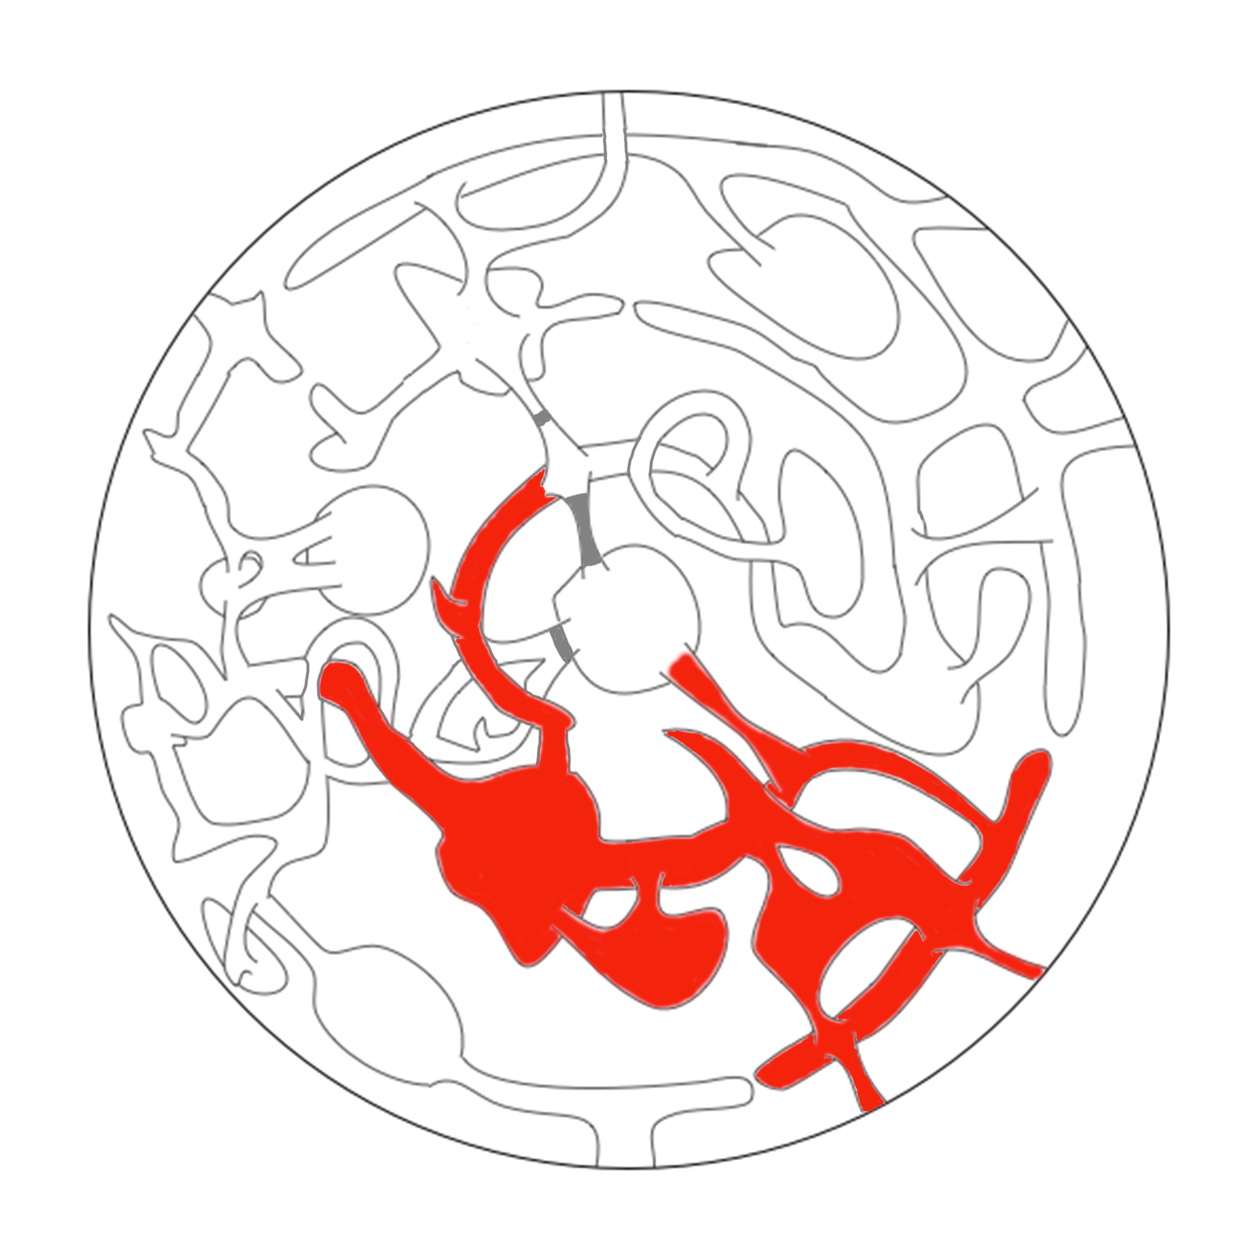
\includegraphics[width=0.7\linewidth]{images/map/2D_map_section_03.png}
	\caption*{Section 3}
\end{figure}

\begin{figure}[H]
	\centering
	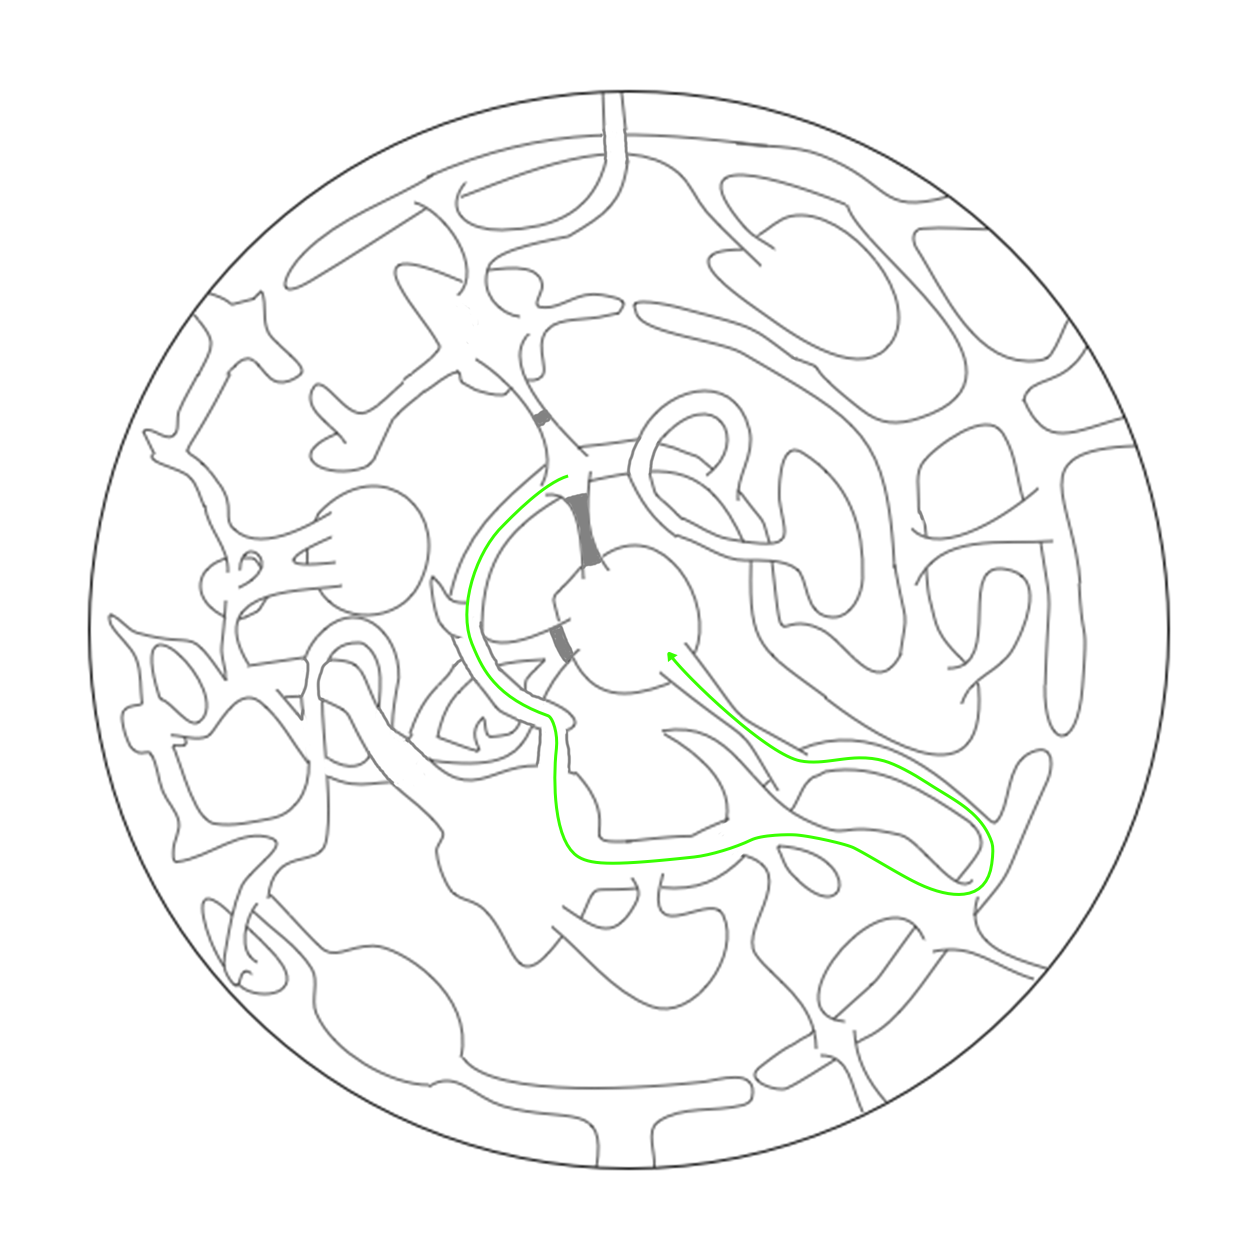
\includegraphics[width=0.7\linewidth]{images/map/map_principle_path_section_03.png}
	\caption*{Section 3 main path}
\end{figure}


\textbf{Encounter}
\begin{itemize}
	\item x1 NeoDemoGorgon
\end{itemize}
Just before entering the room, Elby will have chills down her spine. When Elby and \#010 will enter the den, after a brief iteration between the two, the NeoDemoGorgon will awaken and charge the player aggressively. Upon reaching the 50\% life threshold, the beast will start using the same dimensional travel power as the original one, only limited inside the den. Defeated the beast, Elby will go berserk and starts mutilating the corpse of the NeoDemoGorgon, until \#010 manages to calm her down.

\begin{itemize}
	\item 17 - 50\% Demorat, 30\% Demobat, 20\% Demodog
	\item 18 - NeoDemogorgon x1
	\item 19 - 15\% Demowolves, 35\% Demobat, 50\% Demodog
	\item 20 - 50\% Demorat, 30\% Demobat, 20\% Demodog
	\item 21 - 40\% Demorat, 40\% Demobat, 20\% Demomoles
	\item 22 - 50\% Demomoles, 25\% Demobat, 25\% Demodog
\end{itemize}

\textbf{Sounds}\\
The rustling of moving vines is more intense than Section 2, and a sound similar to the noise of a falling tree can be heard randomly. Elby makes a squelching sound when she walks on a organic branch.

\begin{itemize}
	\item 8 - Monster roar
	\item 9 - Rustling branches
\end{itemize}

\textbf{Lighting}\\
The environment is lit up with a bright red light emitted from the core. The same light shines slightly from the vines coming from the center of the pit, giving the impression of coming from a liquid similar to blood.

\begin{itemize}
	\item 3 - Trigger light change
\end{itemize}

\textbf{Drops}
\begin{itemize}
	\item 18 - Rotten potion
	\item 19 - Fresh potion
	\item 20 - Fresh elisir
	\item 21 - Fresh elisir
\end{itemize}
\newpage


\subsubsection{Giant Chasm Core}
The Core room is located in the center of the Giant Chasm, it has a circular shape with a diameter of 50m. In the center of the room stands the heart of the upsidedown, four times Elby high and at least three times wide, in front of which \#001 awaits the arrival of the player.

\vspace*{0.3cm}
\begin{figure}[H]
	\centering
	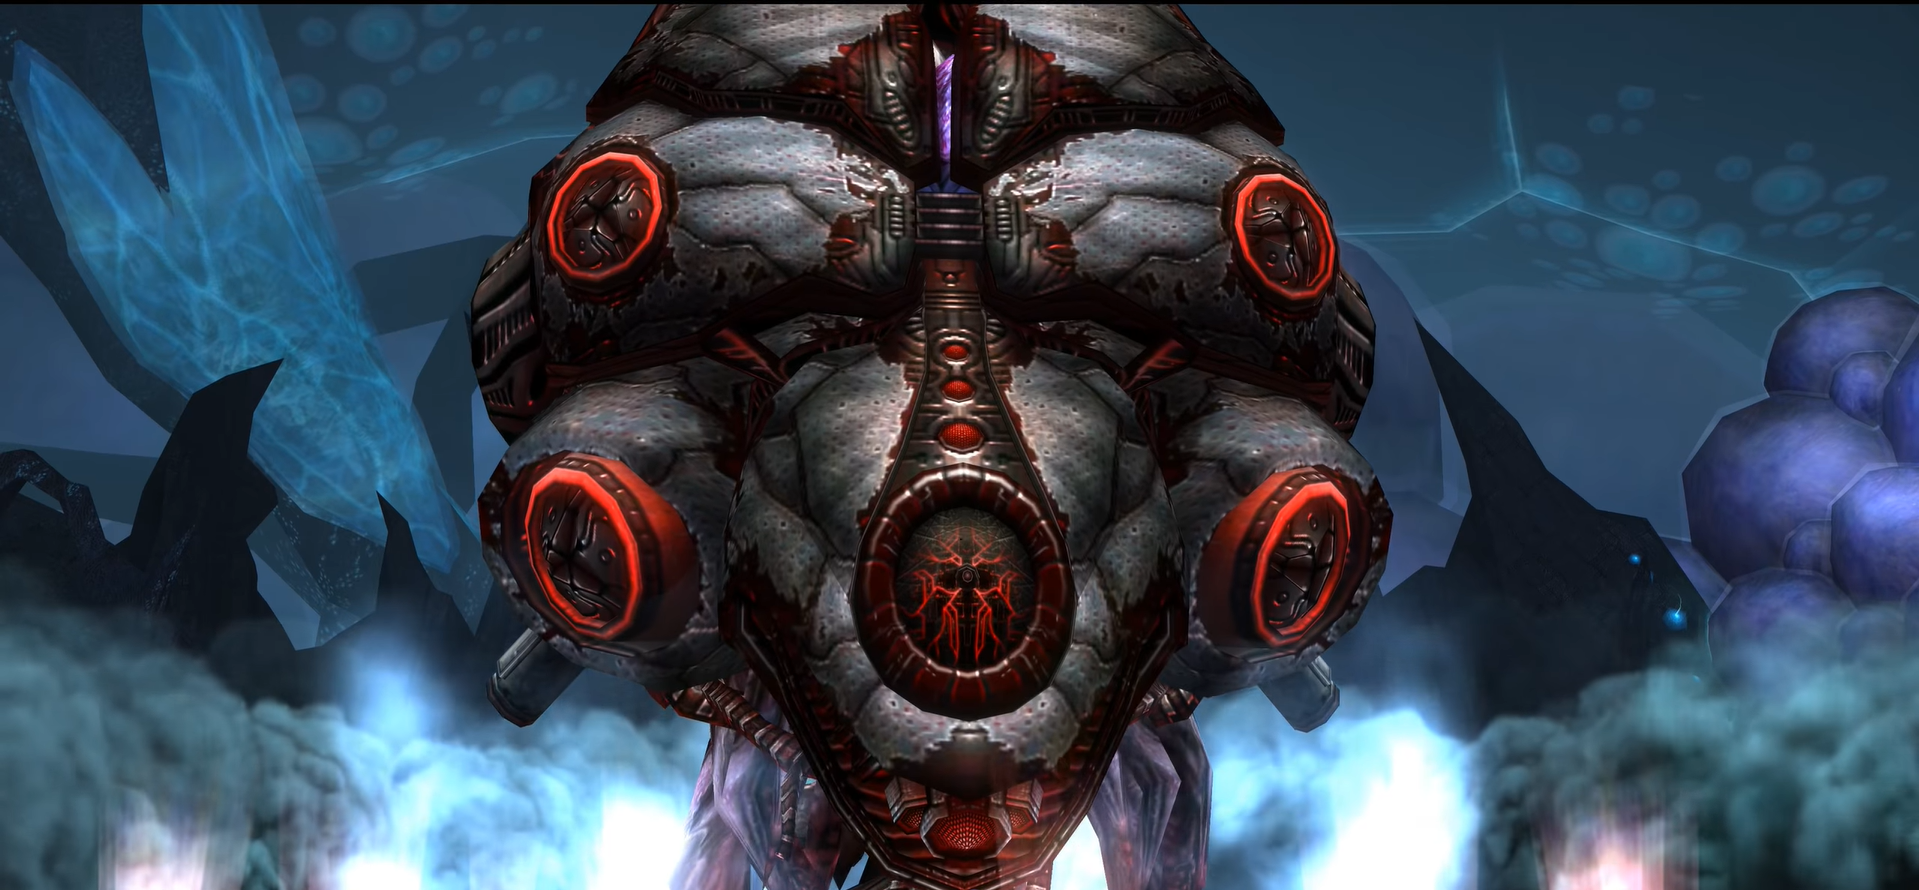
\includegraphics[width=0.8\linewidth]{images/visual_ref/15_giant_chasm/chasm_core.png}
	\caption*{Core of the Upside-Down (in-game it will be more organic and it will emit more red light)}
	\caption{ \textit{[Metroid Prime]}}
\end{figure}

\begin{figure}[H]
	\centering
	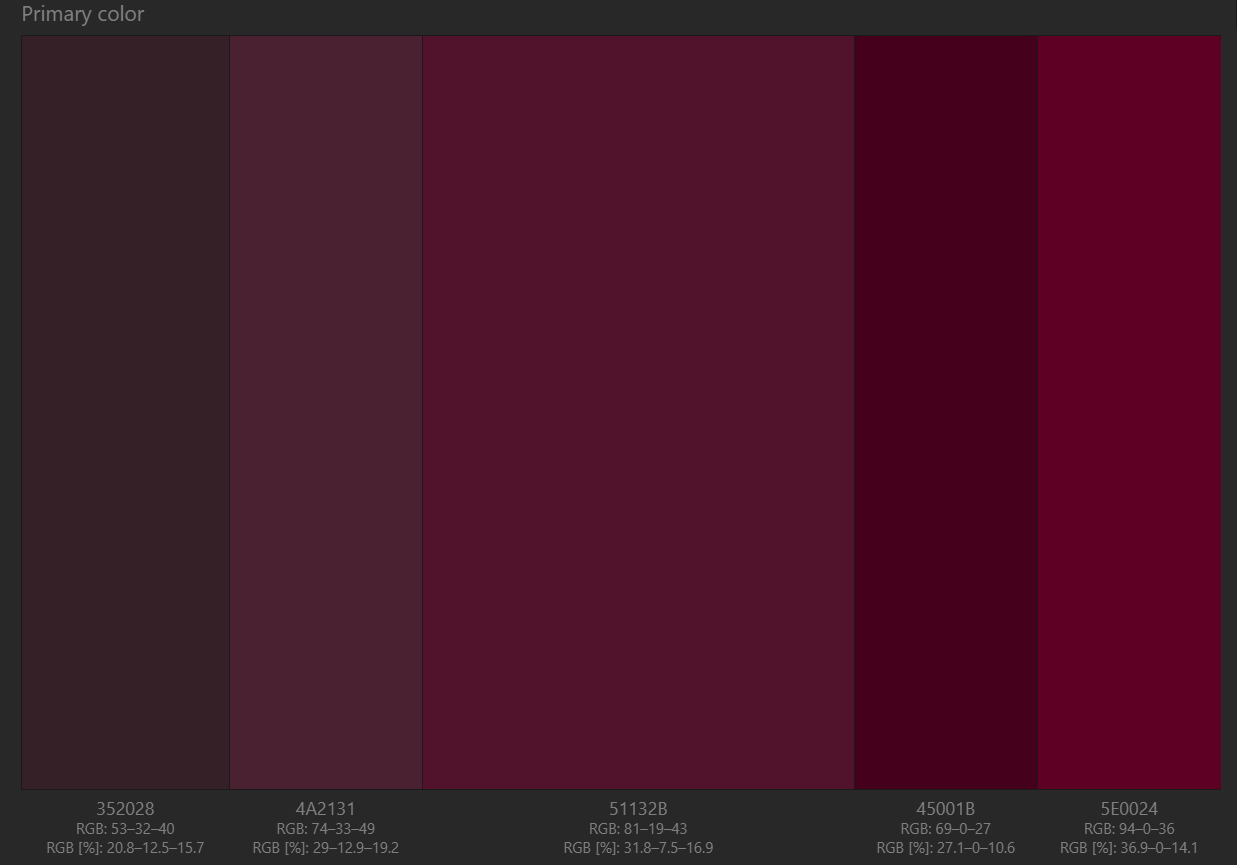
\includegraphics[width=0.8\linewidth]{images/visual_ref/15_giant_chasm/pallette/pallette_section_04.png}
\end{figure}

\begin{figure}[H]
	\centering
	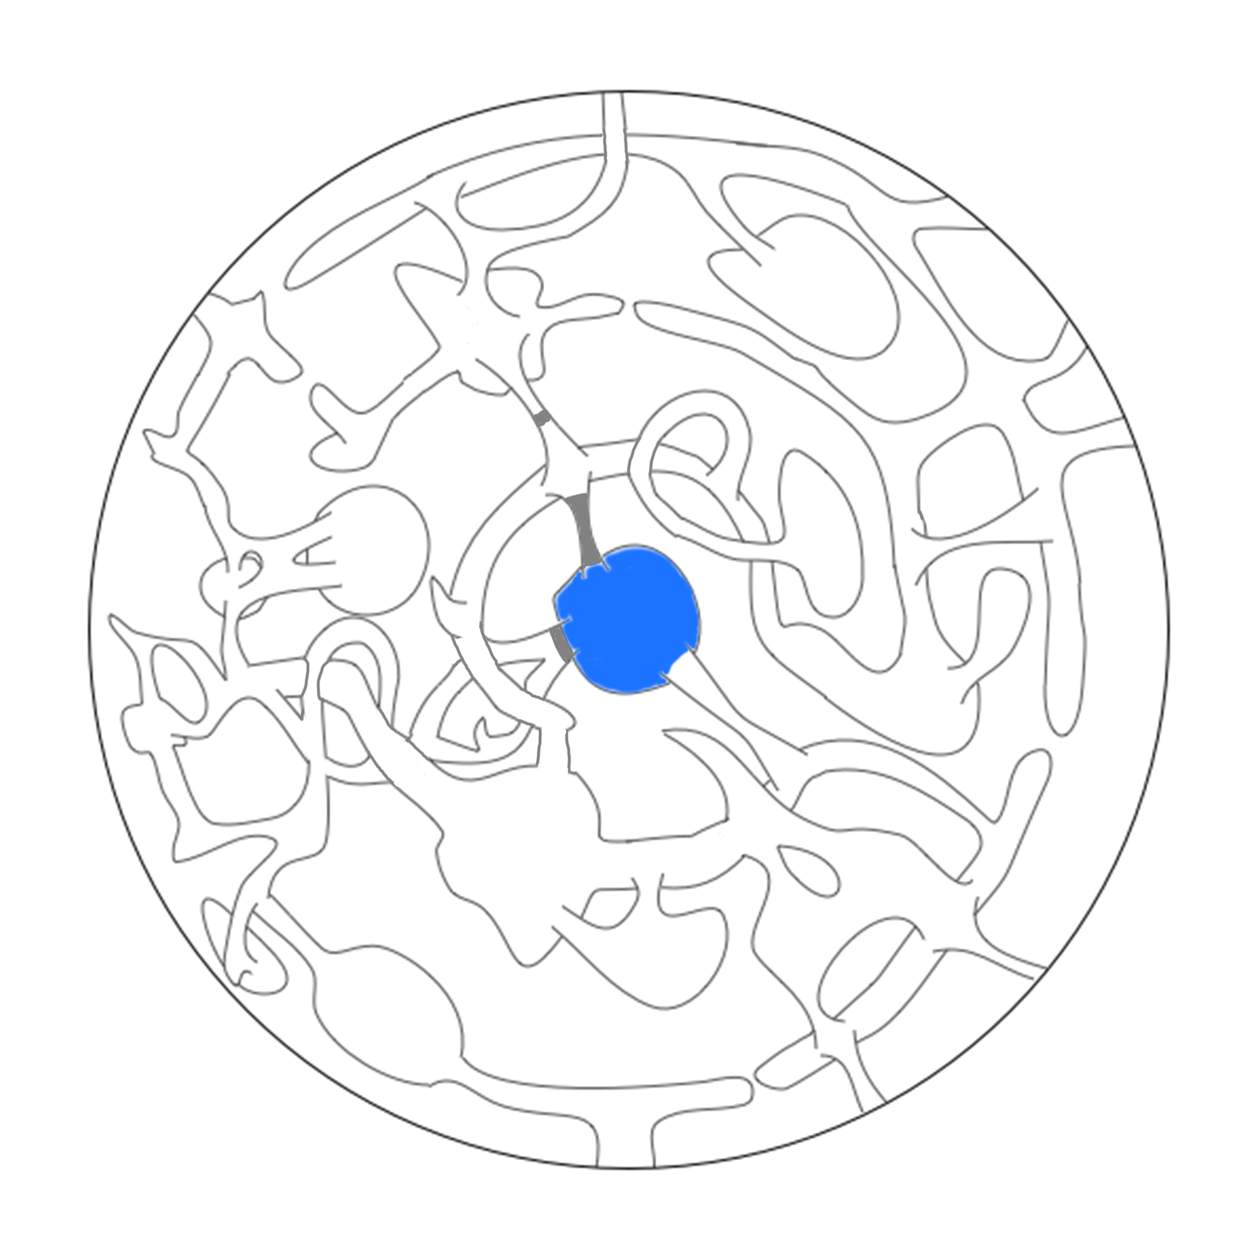
\includegraphics[width=0.7\linewidth]{images/map/2D_map_section_04.png}
	\caption*{Boss room}
\end{figure}
\newpage


\subsection{Dialogues and Level Story}

\subsubsection{Section 1}
\vspace*{0.3cm}

	\textbf{Entered the Giant Chasm, Elby and \#010 remain stunned by the dense network of ramifications that cover the whole area.}

\begin{dialogue}
	
	\speak{\#010} \direct{Astonished} \textit{"So this is the place where the core of the upside-down resides. It looks like a giant crater, it is possible that ..."}
	\speak{Elby} \textit{"I have no time or interest in your hypotheses, we must reach Kyle."}
	\speak{\#010} \textit{"Oh, you're right ... I see a light in the center, I think it's our destination"}\\
	
	\textbf{After a quick inspection, the two decide to continue along the edge and look for a route to the center.}\\
	
	If the player tries to go on the right:
	\speak{\#010} \textit{"This tangle of vines is too thick, we will not be able to pass this way. Let's find another path."}\\
	
	\textbf{Reached the remains of a building that collapsed inside the crater, Elby and 10 arrive in what appears to be
an old ballroom. Suddenly they hear the roars of monsters, which appear one after another around them.}\\
	
	
	\speak{\#010} \direct{Worried} \textit{"We are in their den after all, just try to save as much stamina as possible!"}\\
	
	\textbf{Once the monsters are defeated, they continue along the cliff to reach a second room divided in half
from a pit.}\\
	
	\speak{\#010} \textit{"I don't think I can jump so much, I'm sorry ..."}
	\speak{Elby} \textit{(That branch ... Maybe with my skills I can create a path)}\\
	
	\textbf{After using his telekinesis to cross the pit, Elby and \#010 follow the ramifications to continue on the track until they reach a third room, where they find several monsters impaled by vines.}\\
	
	
	\speak{\#010} \textit{"All these pierced monsters, I think it was \refer{\#001.}"}
	\speak{Elby} \textit{"You should be happy."}
	\speak{\#010} \textit{"Why?"}
	\speak{Elby} \textit{"..."}
	\speak{\#010} \textit{"Ah, if he killed them it means he doesn't have the power to control them, so \refer{\#005} is still alive!"}
	\speak{Elby} \direct{Nods towards \refer{\#010}}\\
	
	
	\textbf{Once at a dead end, they begin to look for a route inland.}\\
	
	
	\speak{\#010} \textit{"This is the only point from which we could descend, but the vines are too thick! Do you have any ideas?"}
	\speak{Elby} \direct{Looks around}
	\speak{Elby} \direct{Indicates a building on the edge of the crater}
	\speak{Elby} \direct{Smiling}\textit{"Freeze it"}
	\speak{\#010} \direct{Excited} \textit{"Maybe by combining our skills we can bring it down. Let's try!"}\\
	
	
	\textbf{After freezing the vines that stabilized the structure and having destroyed them by means of telekinesis, the building begins to collapse and the debris, after rolling along the wall, hit the barrier of vines, opening a gap.}\\
	
	
	\speak{\#010} \textit{"Now we can pass, but let's stay on guard."}
	
\end{dialogue}


\subsubsection{Section 2}
\vspace*{0.3cm}

\begin{dialogue}
	\speak{\#010} \direct{Coff coff}
	\speak{Elby} \textit{"The density of the air has changed, we are getting closer"}\\
	
	Entering the Safe Room:
	\speak{\#010} \direct{Relieved}\textit{"We should be safe in here, we can make a brief stop to regain strength"}\\
	
	Leaving the Safe Room:
	\speak{\#010} \textit{"Let's go, we should be halfway there"}
\end{dialogue}


\subsubsection{Section 3}
\vspace*{0.3cm}


	\textbf{The proximity to the core is increasingly evident: the ground is completely covered with organic vines and the air density is skyrocketing.}

\begin{dialogue}
	
	
	\speak{\#010} \textit{"We're getting closer to the core, the light that emanates is much more intense than before"}
	\speak{Elby} \direct{Angered} \textit{"Don't distract yourself!"}
	\speak{\#010} \textit{"Sorry!"}\\
	
	
	\textbf{Unable to follow the ground path, Elby and \#010 decide to continue the journey using the ramifications of the core as a route}\\
	
	\speak{\#010} \textit{"The branching of the core is extremely dense at this point"}
	\speak{Elby} \textit{"We are almost there"}\\
	
	Section one link, post skill:
	\speak{\#010} \textit{"We can now reach the entrance from here"}
	\speak{Elby} \direct{nods}\\
	
	
	\textbf{Finally they arrive on a non-natural path, certainly created by Kyle to reach the center of the giant chasm.}\\
	
	\speak{\#010} \textit{"\refer{\#001} must be close, are you ready?"}
	\speak{Elby} \textit{"Yes"} or \textit{"Not yet"}\\
	
	If answer is "Yes":
	\speak{\#010} \textit{"Ok, let's go ..."}\\
	
	If answer is "Not yet":
	\speak{\#010} \textit{"Make it quick, \refer{\#005} needs us!"}
	
\end{dialogue}


\subsubsection{Inner Section}
\vspace*{0.3cm}

\begin{dialogue}
	
	\speak{\#010} \textit{"\#001!"}
	\speak{Kyle} \direct{Joking} \textit{"Oh, finally. I was starting to think you were dead along the way!"}
	\speak{\#005} \direct{Squirms}
	\speak{Kyle} \textit{"Hey hey, calm down, wait for your turn"}\\
	
	If the player has visited Kyle's lab:
	\speak{\#010} \textit{"We've been in your lab, we know what you've done and what you are up to!"}
	\speak{Kyle} \textit{"So you found out everything ... Great, you saved me a lot of explanations"}\\
	
	If the player has not visited Kyle's lab:
	\speak{\#010} \textit{"Why all this?"}
	\speak{Kyle} \textit{"I just want back what was taken from me, nothing more"}\\
	
	\speak{\#010} \textit{"And are you going to kill us all for your purpose?"}
	\speak{Kyle} \textit{"Not everyone, just the two of them in case they don't want to cooperate" \direct{Points \refer{Elby} and \refer{\#005}}}
	\speak{Kyle} \textit{"By the way, you are staring at me with a fierce look, do you have something to say?" \direct{Watching \refer{Elby}}}
	\speak{Elby} \direct{Really angered} \textit{"Friends ... don't ... LIE !!!"} \direct{Gust of energy}
	\speak{Kyle} \textit{"Haha, so you consider me a friend, how nice!"}
	\speak{Kyle} \direct{Serious look}
	\speak{Kyle} \textit{"Chatting time's over, now give me your powers!"}
	
\end{dialogue}

\subsubsection{After Boss Fight}
\vspace*{0.3cm}

\begin{dialogue}
	\speak{Kyle} \textit{"... The effect of the core is more intense than I thought ..."}
	\speak{Elby} \textit{"Free \#005. NOW!"}
	\speak{Kyle} \textit{"..."}
	
	\textbf{The costrinctions around 005 are released, allowing him to move.}\\
	
	\speak{\#005}: \textit{"Thank y-"}\\
	
	\textbf{\#005 stops moving and suddenly blood starts to come out of his mouth.}\\
	
	\speak{Kyle} \textit{"You didn't give me a choice."}\\
	
	\textbf{A branch pierces the chest of \#005, extracting a DemoParasite.}\\
	
	\speak{\#010} \direct{Desperate look and vomit from horror}
	\speak{Elby} \direct{Tear from left eye}
	\speak{Kyle} \textit{"And now ..."}
	\speak{Kyle} \direct{swallows the DemoParasite}
	\speak{Kyle} \direct{closes his eyes}\\
	
	\textbf{Elby launches a mental attack, but a barrier of vines block it}\\
	\speak{Elby} "???!!?"
	\speak{Kyle} \direct{Open his eyes}
	\speak{Kyle} \textit{"I have control over the core, there's nothing more you can do."}\\
	
	\textbf{The whole Giant Chasm begins to tremble. In a few moments, hundreds of vines emerge from the ground, trapping Elby and \#010.}\\
	
	\speak{Kyle} \textit{"If you do not want to follow the same fate as \refer{\#005} do not resist and open the portal"}\\
	
	\textbf{A branch wraps around the neck of \#010, starting to strangle him}\\
	
	\speak{Elby} \direct{Initially reluctant} \textit{"Okay. I'll do it ..."}
	\speak{Kyle} \textit{"Great!"}\\
	
	\textbf{Kyle closes his eyes again, entering a state of deep concentration. Suddenly, the air inside the core changes, almost as if all the space there was in a continuos changing state}\\
	
	\speak{Kyle} \textit{"The time is right. Go on!"}\\
	
	\textbf{Elby starts to focus. The chasm begins to tremble again and in few seconds a portal appears in the room. Kyle watches it with a satisfied look and tears running down his face.}\\
	
	\speak{Kyle} \textit{"Now I can finally go home ..."}
\end{dialogue}
